\chapter{Scenarios}
\label{ch:scenarios}
% ##################################################################################################################

\hfill \textbf{Authors:} 
Andreas Horni, 
Marcel Rieser, 
Kai Nagel,
Amit Agarwal,
Hernán Aguirre,
Atizaz Ali,
Rolando Armas,
Joschka Bischoff,
Frederik Bockemühl,
Paul Bouman,
Artem Chakirov,
Christoph Dobler,
Alexander Erath,
Stefan Flügel, 
Eoghan Furey,
Dominik Grether,
Khandker Nurul Habib,
Johan W. Joubert,
Julia Kern,
Benjamin Kickhöfer,
Hubert Klüpfel,
Peter Kucireck,
Gregor Lämmel,
Aonghus Lawlor,
Seungjae Lee,
Milan Lovric,
Michal Maciejewski,
Gavin McArdle,
Andreas Neumann,
Miguel Picornell,
Alexei Pozdnoukhov,
Daniel Röder,
Nicole Ronald,
Waldemar Walerjanczyk,
Adam Weiss,
Elvira B. Yaneza,
Lun Zhang,
Dominik Ziemke

\begin{center} \includegraphics[width=0.7\textwidth, angle=0]{using/figures/MATSimModelsMap} \end{center}

% ##################################################################################################################
This chapter summarizes MATSim scenarios as located on the map in Figure~\ref{fig:scenarios} and listed at \citet[][]{MATSIM-T-Scenarios_Webpage_2014}).

Many scenarios are not public due to data privacy issues. However, knowing about the general methods and approaches adopted for scenario creation and hearing about problems faced thereby might significantly support the building of new scenarios. Content basically covers information on study area, population and demand generation, activity locations, network, simulated modes, calibration and validation, achieved results, associated projects, where to find more, where emphasis is put on specialties of a certain scenario, be it parsimonious data usage procedures, special modules used, or special modes simulated (such as the parataxis in the Gauteng scenario). Some of the scenarios are used since years with a continuous further development. We target at reporting, the latest version. 

Different levels of MATSim involvement are possible. For some regions and projects, MATSim is, for example, only used for traffic assignment whereas for others the complete demand is endogenously handled. Couplings with other forecasting models for transport demand generation have been successfully applied such as the coupling with TASHA for Toronto or the combination of MATSim with the activity-based transport model of Tel Aviv.

\createfigure%
{Scenarios Overview}%
{Scenarios Overview}%
{\label{fig:scenarios}}%
{\includegraphics[width=0.99\textwidth, angle=0]{using/figures/MATSimModelsMap}}%
{}

\clearpage
% ==================================================================================================================
% !TeX root = ../../main.tex
% ##################################################################################################################
\section{Berlin I: BVG Scenario}
\label{ch:scenarios:berlinI}
\hfill \textbf{Author:} Andreas Neumann

\citep[][p.67ff]{Balmer_PhDThesis_2007}

coupling with Visum BVG \\
Marcel: IATBR \\


The Berliner Verkehrsbetriebe (BVG) is Berlin's main public transport company
and runs all kind of services with the exception of the S-Bahn urban rail
system. This includes bus services, the subway network, the largest tram network
of Germany as well as ferry services. The bus network consists of 149
different lines, 6468 directed stops and a vehicle fleet of 1316 buses \citep{BVG2012}.
In total, about 937~million trips were served by BVG in 2012,
41\,\% of them by bus.

% start excerpt from the paper
With the opening of the new international airport of Berlin and Brandenburg BER,
Berlin is expecting some major changes in travel demand. Especially, the
existing airport Tegel, currently exclusively served by buses operated by BVG,
will cease operations. BVG had thus a large interest in a new transport model
for the Berlin area. Due to the big changes, the model should not only deliver
the basis for future planning of the regional transport system, but has to
provide detailed information about passenger flows of different user groups as
well. Such user group specific analyses are considered of high importance for
the BVG in order to provide a basis for their future business strategies, which
is why an agent-based model was specifically requested. Two scenarios were
actually asked for, one for the year 2008 (actual state), and one for the year
2015 (prediction). To fulfill the needs mentioned above, the team of 
\citet{PTV2013}, \citet{Senozon2013} and \citet{VSP2013} at Technische Universit{\"a}t Berlin (TU Berlin)
offered a combined model consisting of both a static macroscopic model built with
PTV VISUM \citep{VISUM2013} as well as an integrated activity-based demand and
dynamic traffic assignment model built with MATSim. During
the project, attention was given that both models were based on the same data
sources and that both modeling processes interact with each other to allow data
exchange between the two models.
% end excerpt from the paper

In
brief, the model contains about 115,000 links, % 113269
about 15,000 directed stops, % 14902
6.0~million agents, % 4422012 (sex) 5992771 (/person)
and 539 public transport lines operated by BVG and other companies of the city
of Berlin and the state of Brandenburg. Among others the model features the transport modes Besides the transport modes car, For a more in-depth description of the
model, its generation and its calibration, the reader is referred to the work of
\cite{NeumannEtAl2014IatbrPtBerlinBook}. The model has been extensively been used in \citet[][Ch 7/8]{Neumann2014PhD} for the development of the minibus module of Section~\ref{sec:paratransit}.



% ################################################################################################################## \cleardoublepage

% ==================================================================================================================
% ##################################################################################################################
\section{Berlin II: CEMDAP-MATSim-Cadyts Scenario}
\label{sec:berlinII}
\hfill \textbf{Author:} Dominik Ziemke

% ##################################################################################################################

As explained in section ?????, transport modeling can be considered as the representation of the interaction of transport demand (i.e. people and goods being transported) and transport supply (i.e. transport infrastructure and services) in the transport system. Depending on the application of innovative strategy modules (see section ?????), MATSim accounts for the adaption of transport demand to transport supply \citep{Balmer2007phd}. It is, therefore, crucial to distinguish choice dimensions, which may be adapted during the modeling process (via the application of innovative strategy modules, see section....) and choice dimension whose initial properties are assumed to be correct (e.g. mode shares have to be initially correct in a scenario where the choice of transport modes is not modeled). In the latter case, it is important that respective properties of the transport demand are correct at the start of the simulation (see section Data Requirements - Demand???).

In order to model these properties of the initial demand correctly, suitable data are needed. A widely utilized source of such data are travel diaries, which contain sequences of departure times, mode choice decisions, and activity locations.
%A disadvantage of using trip diaries is, however, that all information that is taken from the diaries is by definition not sensitive to policy measures. Also, trip diaries are normally only available for a very small fraction of the population. Another drawback is that, in Germany and the U.S. (and many other parts of the world), the geo-coding of the activity location is considered sensitive information under privacy legislation, and thus increasingly difficult to obtain (cite ZiemkeNagelBhat2015).
Many contents of this data source, in particular information concerning locations, are, however, in many parts of the world (e.g. in Germany and the United States) considered sensitive in terms of data privacy legislation and thus increasingly difficult to obtain and to process \citep{ ZiemkeNagelBhat2015IntegratingCemdapMatsimTransferabilityTRB}.

The \textit{Berlin II scenario} (also referred to as the \textit{CEMDAP-MATSim-Cadyts scenario} according to applied models in its setup) is the outcome of an alternative approach that relies exclusively on input data that are freely available and easy to obtain. The starting point for the Berlin II scenario are publicly available commuting matrices which contain home and work places of socially-secured workers on the municipality level. Based on this information, it is possible to model morning and evening commuting peaks.

In order to obtain a demand representation of the full population, two further major modeling steps are required. First, in cases (like in the Berlin case, see below), where the spatial resolution of the commuter matrix is quite coarse, a method to attain origin-destination information at a higher resolution is needed. Second, there needs to be a procedure to model secondary activities, i.e. all other activities that go beyond home and work activities.

The necessity of the first step becomes obvious when looking at the German case, where, for instance, all of the city of Berlin, with 3.4 million inhabitants, is represented by exactly one zone \citep{BA2010Pendlerstatistik}. In the U.S., commuting matrices are typically available only at a county-to-county level. Since such location-aggregation-based matrices may become the rule rather than the exception in privacy-sensitive societies, a (generalizable) method to attain origin-destination information at a higher resolution is needed \citep{ ZiemkeNagelBhat2015IntegratingCemdapMatsimTransferabilityTRB}. The standard solution would be to estimate an activity location choice model. This, however, is difficult if no trip data to estimate the model is available. OD matrix estimation studies \citep{ZuylenWillumsenMatrix-from-cnts} suggest that traffic counts may be used to make an initially rough OD matrix more appropriate for a region. As MATSim is not based on OD flows (see section ????), but on full daily plans, the issue becomes whether there is a procedure to update these initial full daily plans using traffic counts. In the approach to create the Berlin II scenario, a procedure proposed by Flötteröd et al. \citep{FloetteroedBierlaireNagel2010Bayesian} and implemented in the software Cadyts (Calibration of Dynamic Traffic Simulations \citep{Floetteroed2010Manual110}) is applied for this task. Specifically, random draws of possible home and work locations within the home or work municipality given by the commuter matrix are taken. Various MATSim plans each containing one pair of home and work locations are created for each agent. Then, the Cadyts calibration procedure is applied within the iterative MATSim simulation to select those plans, and thus also those locations, which appear more plausible with regard to given traffic counts.

As stated above, however, full daily plans (as opposed to mere home-work-home comuting patterns) are needed. Therefore, the second aforementioned additional modeling step, the modeling of secondary activities for each individual in the region, needs to be addressed. For the Berlin II scenario, the Comprehensive Econometric Microsimulator for Daily Activity-Travel Patterns \citep{BhatEtAl2008CEMDAPUserManual} is used to generate initial complete daily plans for each individual. One the one hand, however, no CEMDAP parameter set is available for Berlin. On the other hand and more importantly, one major goal of the study creating the Berlin II scenario was to show is generalizability \citep{ ZiemkeNagelBhat2015IntegratingCemdapMatsimTransferabilityTRB}. So, the model parameters of CEMDAP estimated for the Los Angeles region (the estimation context) are retained, and then used to generate the initial plans for individuals in Berlin (the application context in the current paper) based on Berlin demographic data.

To sum up, home and work municipalities are taken from the commuter matrix. Within these municipalities, a set of (more precisely spatially defined) potential home and work locations are randomly chosen for each agent. Full daily plans incorporating the various potential locations of each agent are generated with CEMDAP based on a parameter set from another region and local demographic data.

Then, the Cadyts calibration procedure is used to select those initial full daily plans that are most consistent with Berlin traffic count data. In other studies, Cadyts has already been applied to update route choice predictions, both for car \citep{FloetteroedChenEtAl2011BehavioralCalibAndAna} and for public transit \citep{MoyoNagel2013ptNetCalibrationABMTPO}. However, it has not been used to update full daily activity-travel plans, as it has been done in the procedure that created the Berlin II scenario. 

As a result, the Berlin II scenario, is an activity-plan-based MATSim transport model for Berlin that is exclusively based on freely or easily available data. If a commuter matrix, some basic demographics of the population, and traffic counts (or theoretically another suitable data source to run the calibration procedure on) are available for a particular regional context, the approach used to create the Berlin II scenario can be transfered to this context. In fact, the Berlin II scenario itself has to be seen as a \textit{transferred model} because the initial plans generated by CEMDAP are based on parameter estimates from another geographic region (namely the Los Angeles area).

Through a validation based on the Berlin 2008 SrV \textit{System repräsentativer Verkehrserhebungen}, an extensive, regularly conducted travel survey, the quality of the created transport demand representation has been successfully tested. So far, the Berlin II scenario exists for a 1\%{} and a 10\%{} population sample of all persons, i.e. also non socially-secured workers and also non-working people, aged 18 and above for the study region. Currently, only motorized traffic is considered. Stability tests, showing that agents' daily plans keep being chosen when the Cadyts calibration functionality is switched of, have been successfully carried out. This can be seen as a clear indication that the scenario is applicable for policy studies in a meaningful way.

Further improvements like the addition of public transport and a more realistic representation of the population are planned. Moreover, similar approaches of integrating activity-travel pattern generators (e.g. the FEATHERS model, cite?????) with MATSim as a transport simulation are planned.

\ah{NOTES: to be removed:
AN: Szenario entstand aus einer Arbeit zur Nachfragegenerierung. Würde also auch in einen conceptual part passen, anderer Ansatz als die meisten anderen Szenarien ("datensparsam"), Integration von CEMDAP (Modell zur Aktivitätenkettenerzeugung)

Auch link auf Cadyts.

Aktivitätenkettenerzeugung: ähnlich zu Tel Aviv Modell

FEATHERS am Beginn -> Vortrag Wiepersdorf
}

% ################################################################################################################## \cleardoublepage

% ==================================================================================================================
% ##################################################################################################################
\chapter{Switzerland}
\label{ch:switzerland-scenario}
\hfill \textbf{Author:} Andreas Horni

\editdone{This text has undergone the professional edit. Please no grammatical changes anymore! They are most-probably wrong.}

% ##################################################################################################################
The Switzerland scenario was initially created for the project Westumfahrung \citep[][]{BalmerEtAl_ResRep_bdktzrh_2009} and serves as the base for the very frequently used Zürich scenario (Chapter~\ref{ch:zhscenario}). 

Two main branches can be distinguished. The first, older one is based on a one-to-one translation of the Swiss population census \citep[][]{BfS_VZ_2000}; the second applies approaches from the \gls{ipf} family, reported by \citet[][]{MuellerKAxhausen_TechRep_IVT_2013, Mueller_unpub_LATSIS_2012, Mueller_unpub_ETC_2011, Mueller_unpub_STRC_2011, Mueller_unpub_IATBR_2012} to generate population.

The scenario's study area covered all of Switzerland. Due to administrative borders, no demand and supply data were available for adjoining countries, which, then and now, leads to boundary effects; studies focusing on Swiss border areas are difficult.

The population was derived from the Swiss Census of Population~2000 \citep[][]{BfS_VZ_2000}. The complete Swiss population was modeled, resulting in around 7.5\,million agents. 

This population's home locations were given at hectare level and work locations were specified at municipality level from commuter matrices, a component of the Swiss Census of Population~2000 \citep[][p.35]{BalmerEtAl_ResRep_bdktzrh_2009}. A very good overview, in German, of the population generation, its initial individual demand and activity locations can be found in \citet{MeisterEtAl_SVT_2009}. Further information is given in \citet[][]{CiariEtAl_STRC_2008, MeisterEtAl_WCTRS_2010, BalmerEtAl_ResRep_bdktzrh_2009, BalmerEtAl_ResRep_datapuls_2010, BalmerEtAl_HEUREKA_2008}.

Travel demand was basically taken from the 2000 and 2005 National Travel Surveys \citep[][]{BfS-MZ2005_manual_2006} (Swiss microcensus), although this sample substantially underestimated freight traffic and ignored cross-border traffic of non-Swiss residents. Freight traffic for Switzerland was missing at this time (except Zürich, see next chapter). Cross-border traffic was derived from mode-specific, hourly origin-destination matrices given by \citet[][]{VrticEtAl_ResRep_UVEK_2007}. These were disaggregated to around 600\,000 individual \gls{matsim} plans for the whole country, which contain the cross-border traffic originating \emph{outside} Switzerland. Non-Swiss, cross-border traffic starting in Switzerland was supposed to be negligible. 

The activity location data set, comprising home, work, education, shopping and leisure locations, was also derived from the 2000~Swiss Census of Population and the 2001~Federal Enterprise Census \citep[][]{SwissEnterpriseCensus_manual_2001}, providing hectare level information. Facility generation was described in \citet[][p.33]{BalmerEtAl_ResRep_bdktzrh_2009}.

For car traffic, navigation networks from Teleatlas \citep[][]{MultiNet_Webpage_2010} and \gls{navteq} \citep[][]{Navteq_2011} were available. The most-used network was the planning network derived from from the Swiss National Transport Model \citep[][]{VrticEtAl_BiegerEtAl_2003}.

The public transport simulation network was derived from the National Transport Model of the \gls{uvek}, described by \citet[][]{VrticFroehlich_ResRep_UVEK_2010}. 

The scenario simulated car and public transport; schedules for public transport were given at the municipality level. Fine-granular schedules were not available then, but were in preparation. The modes walk and bike were usually ``\gls{teleported}''. 

Calibration was mainly performed for modal split and distance distributions; utility function values were set accordingly.

For validation, count data on city level, cantonal level and national level \citep[][]{ASTRA_Webpage_2006} were available from various sources, resulting in 600\,links measured for Switzerland. An average working day (Monday to Thursday, excluding public holidays) was used for comparisons in current projects.

% ##################################################################################################################
 \cleardoublepage

% ==================================================================================================================
% ##################################################################################################################
\section{Zürich}
\label{sec:zhscenario}
\hfill \textbf{Author:} Andreas Horni

\editdone{This text has undergone the professional edit. Please no grammatical changes anymore! They are most-probably wrong.}

% ##################################################################################################################
The \gls{matsim} team frequently uses the Zürich scenario, based on the Switzerland scenario described above. The Zürich scenario, however, was more detailed; it was enhanced by data available only for the smaller region; \eg traffic light data or freight demand data was only included for Zürich city and the canton. It is under continuous development, calibration and validation and has been applied in numerous projects, serving as a real-world research example.   

\citet{HorniEtAl_TechRep_IVT_2011_a} provided a technical overview of the first scenario branch; \citet[][]{BalmerEtAl_ResRep_bdktzrh_2009} described its generation for the ``Westumfahrung'' project . 

The study area was delineated by a circle, with a 30\,kilometer radius around Bellevue, a central and prominent Zürich location. This delineation led to two versions,  the \emph{Zürich diluted scenario} and the \emph{Zürich cut scenario}. For the first, all agents crossing the study area during the simulated day were considered (Figure~\ref{fig:zurichScenario}), resulting in almost 2\,million agents. For the second, only agents remaining in this area the whole day were modeled. The \emph{Zürich cut scenario} was employed as an experiment in \citet[][]{Hackney_PhDThesis_2009}, but using the \emph{Zürich diluted scenario} for production runs is preferable.

Demand was taken directly from the Swiss model; freight traffic was also added to the Zürich scenario, as follows. Canton Zürich raw freight traffic data was taken from the \gls{kvmzh}, provided by \citet{AMV_Webpage_2011} and documented in \citet[][]{GottardiBuergler_SV_1999}. Zonal level matrices were disaggregated to single \gls{matsim} plans \citep[][]{ShahM_TechRep_IVT_2010}. Matrices for small delivery and heavy trucks were combined into one activity called \emph{freight}. An additional 180\,000 agents were generated for the Zürich region.

For the diluted Zürich scenario, all Swiss facilities, as described above, were used as activity locations. For the diluted scenario, the networks were not thinned out. For  public transport simulation, network and transport schedules were derived from the \gls{kvmzh}. Walk and bike modes were ``teleported''. 

Calibration was mainly done for modal split and distance distributions and utility function values set accordingly.

For validation, count data on city level, cantonal level and national level \citep[][]{ASTRA_Webpage_2006} were available from various sources, resulting in 123\,links measured for the Zürich inner city, delineated by a 12\,kilometer radius around Bellevue. The reduced count analysis radius was applied to reduce boundary effects resulting from demand reduction outside the 30\,kilometer radius study area. An average working day (Monday to Thursday, excluding public holidays) was used for comparison in current scenarios.

Some traffic signal data was available for Zürich city \citep[][]{STAPOZH-DAV_unpub_gtZH_2008}; this was integrated for the Westumfahrung project.
%
\createfigure%
{The diluted Zürich scenario}%
{The diluted Zürich scenario}%
{\label{fig:zurichScenario}}%
{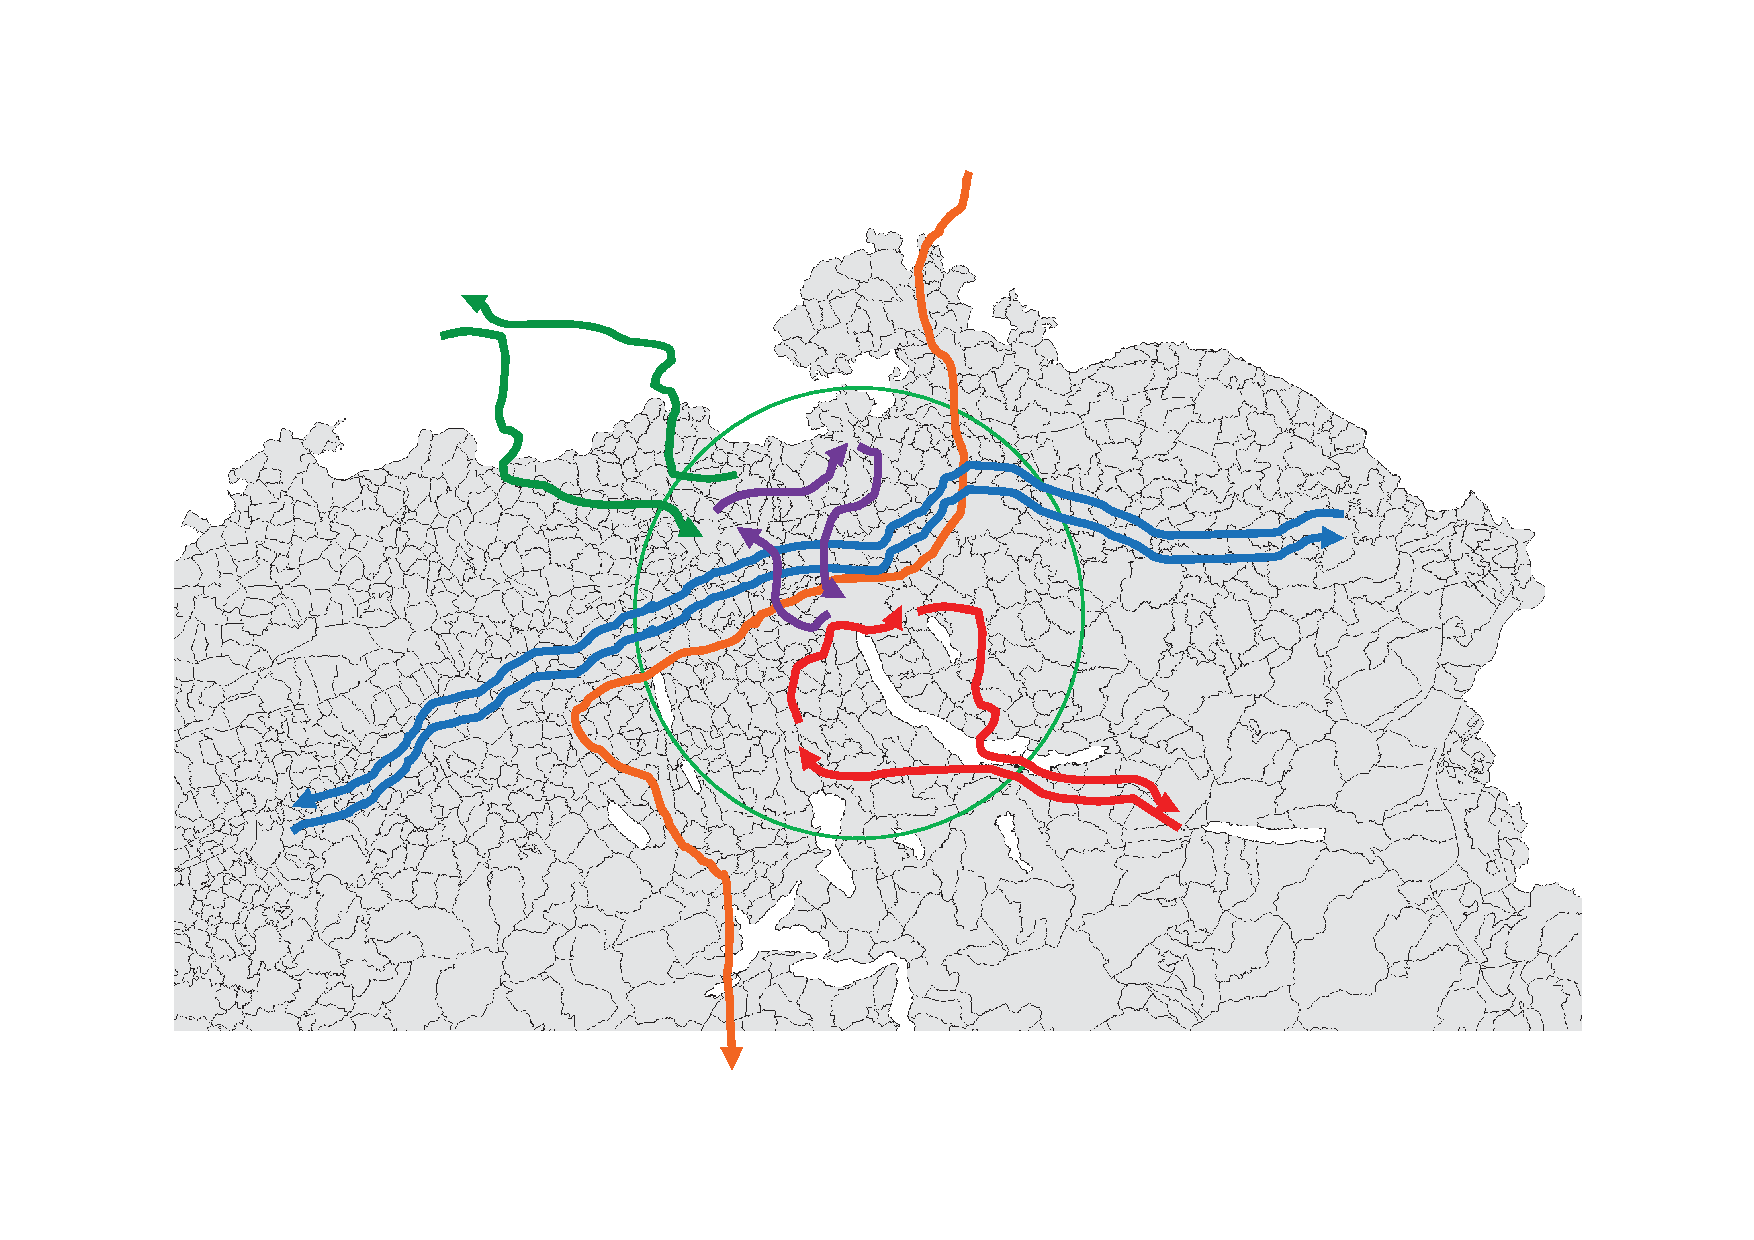
\includegraphics[width=0.99\textwidth, angle=0]{using/figures/zh.pdf}}%
{}

% ##################################################################################################################
 \cleardoublepage

% ==================================================================================================================
% ##################################################################################################################
\section{Singapore}
\label{sec:singapore}
\hfill \textbf{Author:} Alexander Erath, Artem Chakirov

% ##################################################################################################################
The MATSim Singapore scenario \citet[][]{ErathEtAl_TechRep_FCL_forth} was implemented and is maintained at the Future Cities Laboratory, a research program of the Singapore-ETH Centre for Global Environmental Sustainability (SEC) and part of Singapore's National Research Foundation CREATE (Campus for Excellence and Technological Enterprise). The scenario covers the whole area of Singapore with a population of approximately 5 million inhabitants and includes traffic from and to neighboring Malaysia. Singapore provides an excellent study case for an agent- and activity based modeling approach: a fairly densely populated city with an extensive public transport infrastructure and advanced transportation and pricing policies. 

% ====================================================================================================
\subsection{Demand}
In the absence of a full-population census for Singapore, a synthetic population is generated based on data from the Household Interview Travel Survey (HITS) 2008 \citep[][]{Choi_JOUR_2010} and population breakdowns of Singapore’s population census 2010. The synthetic population was derived using the fitting and sampling method \citep{MuellerKAxhausen_TRB_2011}, where a reference sample of household and person records  is weighted using an iterative proportional fitting (IPF) technique, until the weighted sample matches marginal control totals from the census. In our case, the reference sample is the records form the travel survey, and the fitting technique is the entropy optimization method proposed by \citet[][]{BarGeraEtAl_TRB_2009}, implemented by Kirill Müller, IVT, ETH Zürich. Then the reference sample records are replicated through weighted sampling until the population total is met. 
 
Car ownership is modeled on a household level and driving licenses are assigned to individuals, using discrete choice methods. Given the high taxation of cars in Singapore, the model reflects that car ownership is much lower than in other developed nations. The model presented in \citet[][]{VanEggermondEtAl_IATBR_2012} includes not only socio-economic but also spatial variables and has proven to be essential to the MATSim Singapore model, leading to accurate mode choice and mode share predictions. 

Activity locations are defined on the level of individual buildings, with the information on building and facility types compiled from various sources such as the land-use master plan \citep[][]{URA_Rep_URA_2008}, government websites and online directories as well as points of interest information provided by NAVTEQ. In the absence of a business census, an innovative approach for identification of locations and corresponding number of work places has been developed. It draws from the full smart card data record of public transport journeys and enriches it with information on land-use and estimates of building floor space. In a first step, a probabilistic model is applied to a daily record of public transport journeys in order to identify types of activities performed between two subsequent public transport trips. Estimated and calibrated using HITS 2008 records, the model combines variables such as time of day, activity duration and land-use around each stop or station to ensure an accurate differentiation between home, work or other activities. After accounting for mode shares in 53\,different zones, an optimization technique employing accessibility computation is applied in order to distribute work activities to individual buildings. More details on the newly developed methodology and its practical application are reported in \citet[][]{ChakirovErath_IATBR_2012} and \citet[][]{OrdonezErath_TRR_2013}. 

The assignment of households to buildings is performed using detailed information on residential developments: for public housing which represent about 80\,\% of Singapore's residential building stock, information on the distribution of different dwell types is employed, while for privately owned condominiums, only information on the number of apartments per building is available. Work locations are assigned using a zone-based gravity model that uses the prior estimated number of work activities in each building as additional information for the distribution of workplaces within each zone. Activity chains are assigned based on their observed frequency in HITS, taking into account key socio-demographic parameters such as sex, age, occupation and income. Activity chains of type home~--~work~--~home are by far the most frequent, accounting for approximately 50\,\% of the trips.
Freight and cross border traffic as well as tourist travel demand are derived based on a set of origin destination matrices provided by the Singapore Land Transport Authority (LTA). These matrices are converted into special daily plans. Information on the temporal distribution of trips for freight is derived from loop detector data for freight and temporal attraction profiles of major tourist sites.

% ====================================================================================================
\subsection{Supply}
Using a semi-automatic map-matching algorithm~\ref{sec:networkeditor-singapore} a high-resolution navigation network provided by NAVTEQ is map-matched to and enhanced with lane and capacity information from the Land Transport Authority's (LTA) planning network. In absence of access to traffic signal cycle time data, traffic lights are not specifically modeled. Extensive attention was paid to the modeling of public transport due to the the importance of interaction between private and public transport in Singapore’s context of high density and limited space. Simulating dynamic effects such as bus bunching is crucial for obtaining realistic travel times and mode shares. Public transport network and schedule data provided by LTA includes bus and train routes,  as well as the location of stops and stations. This information has been matched to the road network using yet another map-matching algorithm presented by \citet[][]{Ordonez_HKSTS_2011, Ordonez_Webpage_2011_4}. More recently, the scenario got updated by using public transport schedule data as derived from public transport smart card data records \citet[][]{Fourie_TechRep_FCL_2014}. Such schedule information accounts for the actual vehicle dispatch frequencies and headways, which undergo continuous adjustments and in some cases can substantially deviate from the published schedule. Furthermore, additional features of the public transport simulation in Singapore’s model include advanced bus dwell time model \citep[][]{SunEtAl_TransResA_2014} as well as an approximation of the distance based public transport fare scheme.

Other modes, specifically walking and cycling are "teleported" with constant travel speeds and without any interaction with other users. 

% ====================================================================================================
\subsection{Behavioral parameters}
The behavioral parameters, specific to Singapore's context have been borrowed form the study by \citet[][]{LTA_unpub_2009} and used in conjunction with the widely applied Charypar-Nagel function for activity scoring \citet[][]{CharyparNagel2005ga4acts}. Thereby same parameters have been used for all agents, neglecting heterogeneity of user preferences and values of time in the initial scenario implementation. Furthermore, no additional crowding penalties accounting for travelers' discomfort have been considered at this stage and the effects of public transport overcrowding are only taken into account with the physical vehicle capacity limitations as well as its implications on dwell time and occurrence of the bus bunching phenomenon. 

% ====================================================================================================
\subsection{Policy}
The MATSim model for Singapore also includes the Electronic Road Pricing (ERP) scheme featuring time and vehicle dependent road pricing. Based on two data sets indicating the location and time dependent price levels, prevailing tolls are specified for 73\,network links where toll gantries are installed as of February, 2012. To account for the widely available dedicated bus lanes, additional links that are attributed to be used exclusively by buses have been added to the network. The capacity of the respective existing links has been reduced accordingly, even if in some cases the exclusive use of dedicated lanes by buses is granted during the peak hours only. Such a simplified setup, insensitive to the time dynamic operation of the dedicated lanes, leads to an underestimation of actual road capacity during periods when bus lanes are also open to other motorized traffic. However, as most links featuring bus lanes consist of three or more lanes, the effect on modeled traffic conditions during off-peak hours appears to be low.

% ====================================================================================================
\subsection{Calibration and validation}
Road usage data is available for around 200\, 
%\textbf{EXACT 200?} 
count stations in hourly intervals. The availability of public transport smart card data provides an additional dimension for validation. In particular opening of new mass rapid transit (MRT) lines since setting up the model in 2012 presents a unique opportunity for comparison the observed ridership with predicted ridership in the model. However, systematic calibration and detailed validation are yet to be conducted.

% ################################################################################################################## \cleardoublepage

% ==================================================================================================================
% ##################################################################################################################
\subsection{Munich, Germany}
\label{ch:scenarios:munich}
\hfill \textbf{Author:} Benjamin Kickh\"ofer

The \acrshort{matsim} scenario for the Munich metropolitan area was set up during the year 2010.%
%
\footnote{
%
The most detailed descriptions of the scenario can be found in \citet{KickhoeferEtAl_VanoutriveVerhetsel_2013} and \citet{Kickhoefer_PhDThesis_2014}.
%
}
%
The main goal was, and still is, the simulation of local air pollutant and global greenhouse gas emissions, and how their levels change with respect to different policy measures -- on aggregated and spatially disaggregated level. The scenario was therefore used for the development and testing of the \gls{emt} (see Ch.~\ref{ch:emissions}).

Network information from \acrshort{visum} was converted into \acrshort{matsim} format, resulting in a network of 17'888 nodes and 41'942 links.
%
This transport supply was then linked to travel demand from different sources: an activity-based demand for inner-urban traffic from survey data was created based on "Mobility in Germany" \citep[MiD 2002,][]{FollmerEtAl_TechRep_infasDIW_2004}. This part of the synthetic population consists of roughly 1.4m individuals with detailed vehicle information for every household.
%
Commuter and reverse commuter were modeled based on data provided by the German Federal Employment Office \citep{BoehmeEigenhueller_TechRep_IAB_2006}. This part of the population consists of roughly 0.5m individuals from which 0.3m commute to Munich for work. The remaining individuals live in Munich and commute to their workplace in the surroundings of Munich.
%
Freight traffic was also introduced into the model by using data from the German Ministry for Transport \citep{ITBBVU_TechRep_2007}. This part of the population consists of roughly 0.15m freight vehicles who perform one single commercial trip per day.

The scenario has so far been used for several case studies:
%
\citet{HuelsmannEtAl_LAS_2011} used a single street corridor of the scenario to validate simulated travel times and emission levels against actual data obtained from a test vehicle.
%
\citet{KickhoeferEtAl_VanoutriveVerhetsel_2013} investigate the relationship between the price elasticities of car travel demand and those of air pollutant emissions.
%
\citet{HuelsmannEtAl_GerikeEtAl_2013} identify areas with high air pollution concentration in the city. They define these areas as 'hotspots' since the \gls{eu} limits for \gls{no2} are exceeded. The authors then incrementally raise the toll levels for passing the hotspots until they disappear in order to estimate the true avoidance costs of the \gls{eu} threshold values.
%
\citet{KickhoeferEtAl_NSE_2013} derive time-dependent vehicle-specific first-best air pollution tolls in order to create a benchmark for the evaluation of real-world policies.
%
\citet{KickhoeferKern_MobilTUM_2014} go a step beyond and calculate time-dependent vehicle-specific air pollution exposure tolls in order to correct the toll levels by \citet{KickhoeferEtAl_NSE_2013} for the number of affected individuals.



% ################################################################################################################## \cleardoublepage

% ==================================================================================================================
% ##################################################################################################################
\section{City of Sioux Falls, South Dakota}
\label{ch:scenarios:siouxfalls}
\hfill \textbf{Author:} Artem Chakirov

The Sioux Falls scenario represents a small scale scenario featuring realistic demand with socio-economic and demographic attributes and an integrated public transport system. Based on the  Sioux Falls road network commonly featured as a test-case in the transportation literature \citep[][]{BarGera_TNTP_Webpage_2013}, the scenario aims to provide a fully dynamic demand with heterogeneous users and a high degree of spatial resolution. It can serve as a convenient test-case for the study of different transportation policies as well as a test bed for the software extension and development. However, it is important to stress that despite the use of real world data for its generation, the scenario does not aim to replicate the real City of Sioux Falls in South Dakota, US and remains a fictitious test-case scenario. Detailed report on scenario generation and its characteristics is provided \citet[][]{ChakirovFourie_TechRep_FCL_2014} and can be found at www.matsim.org/scenario/sioux-falls. 

Often used test scenario . Not aimed at replicating the real City of Sioux Falls, South Dakota.

% --------
\paragraph{Demand:}

A realistic, socio-economically and demographically diverse demand population with  heterogeneous preferences is crucial for unlocking the full potential of an agent-based simulation. However, the generation of a disaggregated, agent-based demand description, which closely resembles reality, not only in terms of trip origins and destination, but also with respect to associating travel patterns with socio-demographic characteristics, is challenging.

In order to address this challenge in case of Sioux Falls scenario and represent the household structure, demographic profile and income distribution as realistically as possible, a synthetic population of households using entropy maximization technique is generated. It matches the aggregate distribution of demographic attributes (age, sex and household income) recorded during the 2010 US Census for the 27 census tracts inside and adjoining the city centre of Sioux Falls and is composed of household and person records taken from the (anonymous) 5-year sample (2007-2011) of the American Community Survey, covering 5.0\% of all households.

On the demand side of the activity-based model only two simple activity chains are initially included, in order to keep the scenario accessible and to facilitate interpretation and understanding of the possible effects of policies under study. Modelling only home – work – home and home – other – home activity chains, destinations are assigned using a parameter-free radiation model (Simini et al. 2012).

Activity locations are identified using the data set of real building stock provided by the City of Sioux Falls GIS division. The home location of each household is assigned randomly to a residential unit within the tract it belongs to. As no information on the real number and distribution of work places within the relevant area is easily accessible, the static OD-Matrix from LeBlanc et al. (1975) are taken as an indicator of workplace attraction for each zone. Subsequently, the assignment of work places to individual workers was performed using a parameter free radiation model presented by Simini et al. (2012).

In order to exploit the full potential of a disaggregated demand and to add another degree of realism to the scenario, a car ownership model is applied to the synthetic population of households. An ordered probit model estimated by Giuliano and Dargay (2006)based on the US Nationwide Personal Transportation Survey (NPTS) 1995. Next to socio-demographic characteristics of a household (number of adults, children, pensioners, household income), the model uses attributes of residential location (population density, public transport access and dwelling type), which allows to better account for characteristics of the Sioux-Falls scenario with its added area-wide bus network. 

% --------
\paragraph{Supply:} 

A transportation test network should ensure sufficient complexity of travellers’ choice dimensions while limiting computational effort. To this end, the Sioux Falls test network was introduced by Morlok et al. (1973) and later adapted as a benchmark and test scenario in many publications, as e.g. LeBlanc et al. (1975), Abdulaal and LeBlanc (1979a), Suwansirikul et al.  (1987), Friesz et al. (1992), Meng et al. (2001), Bar-Gera et al. (2013) to name but a few. The structure of this network captures the major arterial roads of the City of Sioux Falls, but was never intended to replicate the real city or all characteristics of its transportation system, such as travel times or mode share. The network os comprised of 76 arcs, 24 nodes and 552 origin-destination pairs. For this scenario the capacities of the roads were adjusted according to values provided by the Highway Capacity Manual (TRB, 2000) or other related research publications (e.g. Ng and Small, 2011). The public transportation network includes 5  bus lines, as initially proposed by Abdullal and LeBlanc (1979), with bus stops placed in constant distance of 600m away from each other. 

Due to the design of MATSim’s queue simulation, agents are only handled at the beginning and end of each network link, and cannot enter or leave a link along its length. Therefore, origins and destinations located along very long links will lead to a loss of spatial detail, as all origins and destinations along the length of the link are effectively assigned the same coordinate. Consequently, to improve the level of spatial detail, all links of the Sioux Falls network are evenly split into smaller links with maximal length of 500 meters each. Following this operation, the network detail increased from 27 to 282 nodes and the number of links increased from 76 to 334.

In addition to car and bus modes, walking as 'teleported' mode with constant travel speeds and without any interaction with other users is used as the non-motorized mode of transportation. 

% --------
\paragraph{Behavioural parameters:}

The behavioural parameters used in utility functions of activities and trips are based on the estimated demand model for Sydney by Tirachini, Hensher, and Rose (2012). The time-related parameters derived in their model have to be adjusted for application in the activity-based context. In order to provide a value for marginal utility of performing an activity, the travel mode with smallest disutility is set as a baseline, under the assumption that travelling with this mode is as good or as bad as idling and doing nothing. Therefore, the corresponding parameters are split into opportunity costs of time and a mode-specific disutility of travelling, as was done previously by Kickhöfer et al. (2011), Kickhöfer et al. (2013), Kaddoura et al. (2013), Kickhöfer and Nagel (2013), who employed the same parameters within their MATSim based studies. 

% --------
\paragraph{Results, drawbacks and outlook:}

The stability and performance of the Sioux Falls scenario has been tested using two set of activity timing constrains as well as 5 different random seeds. which all delivered stable and realistic results. Furthermore \citet[][]{ChakirovFourie_TechRep_FCL_2014} also investigate the existence and shape of the Macroscopic Fundamental Diagram, as demonstrated by Geroliminis and Daganzo (2007, 2008). 

However, the more recent experience has shown certain drawbacks of the coarse network representing only major arterial roads and neglecting finer neighbourhood access road network. Combined with the realistic synthetic population and high demand peaks during rush hours, the network appears to be sensible to network breakdowns under high loading conditions. 

Along with the coarse road network, the coarse level of public transport network and therewith its low level of accessibility and attraction represents another drawback, in particular relevant for simulation and evaluation of policies sensible to or requiring certain share of public transport users. 

Substituting, the original Sioux-Falls networks with its only 76 links with a finer Open Street Map network and adding additional public transport line to it, allows to address this problem, but brings another drawbacks at the same time. First, it increases time and resources for routing and dynamic queue simulation due to the significantly larger number of links and nodes present in the network. Second, the increase in total network capacity leads to the disappearance of congestion during peak hours.

The extended simulation times can be improved by using the new pseudo-simulation methodology, currently developed by Fourie (2014). The larger network capacity can be addressed by the inclusion of freight and through traffic into the scenario. 

Drawbacks: course resolution of the network
public transport is not attractive and accessible enough, especially for experiment design in european context
no freight of through traffic


% ################################################################################################################## \cleardoublepage

% ==================================================================================================================
% ##################################################################################################################
\subsection{Barcelona}
\label{ch:scenarios:barcelona}
\hfill \textbf{Author:} Miguel Picornell

zugesagt

% ################################################################################################################## \cleardoublepage

% ==================================================================================================================
% ##################################################################################################################
\section{Brussels}
\label{ch:scenarios:brussels}
\hfill \textbf{Author:} ?


% ################################################################################################################## \cleardoublepage

% ==================================================================================================================
% ##################################################################################################################
\chapter{Cottbus: Traffic Light Simulation}
\label{ch:cottbus}
\hfill \textbf{Authors:} Joschka Bischoff, Dominik Grether

\editdone{This text has undergone the professional edit. Please no grammatical changes anymore! They are most-probably wrong.}

% ##################################################################################################################
The Cottbus (Germany) scenario (Figure~\ref{fig:scenarios:cottbus_location}) is used for traffic light simulation (see Chapter~\ref{ch:signalslanes}). 
It is explained well in \citet[][pp.~87]{Grether_PhDThesis_2014}; this chapter briefly reviews the main points. 
The scenario data is generally available to the public.

The network is derived from \gls{osm} data in summer, 2010 \citep{Bischoff2010BaSylvia} and 
covers all streets within the city boundaries, as well as main roads in the surrounding Spree-Neiße administrative district . 
It is designed as a 100\,\% sample. 
The population is based on the German federal employment agency commuter statistics for both Cottbus and Spree-Neiße \citep{WiethoelterBogaiCarstensen2010IABPendlerberichtBB}. 
As such, the population has only home-work-home plans spread over the usual commuting times, resulting in two peaks, including 
33\,479 agents traveling exclusively by car. 
The scenario is generally not very busy; the area does not usually have major congestion issues.

Figure~\ref{fig:network_municipalities_cottbus_landuse} shows the network over the 
``Corine Land Cover'' landuse \citep{CorineLandCover2006Data}, provided by European Environmental Agency. 
Woods and agricultural areas are depicted; most of the region is agricultural use area.  
Virtual persons in \gls{matsim} need a geographic coordinate for their activities. 
If this coordinate is drawn randomly (solely based on municipality borders), home and work activity locations are uniformly distributed over  the area, \ie most of them in woods and fields. 
Thus, activity locations are drawn randomly in combination with land use data. 
The coordinate must be in the municipality area and for home activity, it must be located in urban fabric areas; for work locations, industrial or commercial areas are also allowed. 
The resulting home activity locations are shown in Figure~\ref{fig:cottbus_population_home}. 

The scenario contains data for 22\,traffic signals within the city center, based on the city's 2009~signal plans; junction layout is also modeled in detail. Fixed-time control data is taken from \citet{KoehlerStrehler2010SignalDemandOptimization}.  
Due to higher transport network resolution, several originally recorded fixed-time control schedules are invalid and were removed; data for 22\,junctions is available. 
Figure~\ref{fig:cottbus_network_signal_locations} shows their transport network location.  

Public transit, not part of the original scenario, is available based on 2011~schedules, although it is not currently used. 
\createfigure%
{Cottbus scenario: Geospatial location within Germany, Europe}%
{Cottbus scenario: Geospatial location within Germany, Europe}%
{\label{fig:scenarios:cottbus_location}}%
{%
  \createsubfigure%
	{Geospatial area of Brandenburg within Germany, Europe (Red); City of Berlin (Yellow)}
	{\includegraphics[width=0.49\textwidth]{./scenarios/figures/brandenburg_europe.png}}
	{\label{fig:scenarios:cottbus_brandenburg_europe}}
  \createsubfigure%
	{Geospatial area of Cottbus (Dark Red), within administrative district Spree-Neiße, Brandenburg (Light Red)}
	{\includegraphics[width=0.49\textwidth]{./scenarios/figures/brandenburg_spree_neise_cottbus.pdf}}
	{\label{fig:scenarios:cottbus_bb}}
}%
{\citet{Grether2014PhD}}

\createfigure%
{Cottbus scenario: Network and population}%
{Cottbus scenario: Network and population}%
{\label{fig:cottbus_network_population}}%
{%
  \createsubfigure%
	{Cottbus network and municipality borders}
	{\includegraphics[width=0.49\linewidth]{./scenarios/figures/2013_network_gemeinden_landuse_edit.pdf}}
	{\label{fig:network_municipalities_cottbus_landuse}}
  \createsubfigure%
	{Synthetic population for the Cottbus scenario, geospatial location of home activities}
	{\includegraphics[width=0.49\linewidth]{./scenarios/figures/2013_network_gemeinden_landuse_population_home.jpg}}
	{\label{fig:cottbus_population_home}}
}%
{Source:~\citet{Grether2014PhD}} 

\createfigure%
{Cottbus scenario: Network, area with traffic signals within the city of Cottbus}
{Cottbus scenario: Network, area with traffic signals within the city of Cottbus}
{\label{fig:cottbus_network_signal_locations}}
{%
  \createsubfigure%
	{Location within city of Cottbus}
	{\includegraphics[width=0.49\linewidth]{./scenarios/figures/2013_cottbus_network_signals.jpg}}
	{\label{fig:cottbus_network_signals}}
  \createsubfigure%
	{Signalized area in detail}
	{\includegraphics[width=0.49\linewidth]{./scenarios/figures/2013_cottbus_network_signals_zoom.jpg}}
	{\label{fig:cottbus_network_signals_zoom}}
}%
{\citet{Grether2014PhD}}

% ##################################################################################################################

% Andreas Neumann-Mail: frei verfügbar. ÖV vorhanden, 100\% Szenario, das sich mit einigermassen geringem Aufwand rechnen lässt. Grundlage für Dominik G.s Ampelpart
  \cleardoublepage

% ==================================================================================================================
% ##################################################################################################################
\section{Dublin}
\label{sec:dublin}
\hfill \textbf{Authors:} Gavin McArdle, Eoghan Furey, Aonghus Lawlor, Alexei Pozdnoukhov

% ##################################################################################################################
\subsection{Introduction}
In order to demonstrate a new spatial choice model, a micro-simulation of urban traffic flows for the Greater Dublin Region was implemented using MATSim. The scenario simulates leisure activities and commuting trips completed by individuals using private cars over a twenty four hour period. For commuting trips, detailed information from the Irish Census was used while a new spatial choice model, inspired by the radiation model, was developed for leisure trips. The effectiveness of the approach was validated using hourly data from count stations on the main motorways around Dublin City. The results show that the micro-simulation accurately reproduces traffic volumes.

% =======================================================================================
\subsection{Study Area}
County Dublin, in Ireland covers an area of approximately 115\,square kilometers and encompasses several administrative areas. Dublin is a coastal county with the Irish Sea lying to the East of the county. In order to capture both intra-city and inter-city flows, the scenario considers individuals who live or work in the Dublin. This captures those who commute into or away from Dublin as well as those who reside and work there.

% =======================================================================================
\subsection{Network}
To capture the desired study area for the scenario, the network consists of all roads in the Greater Dublin Region and the major roads for the remainder of the county. The road network consists of a mix of motorway, national routes and local roads. The road network was extracted from Open Street Map (OSM) along with other information such as the speed limits and number of traffic lanes. This OSM network was prepared for use in MATSim. Private vehicles were the focus of this study and so the public transport network was not considered but can be incorporated into the micro-simulation in future studies.

% =======================================================================================
\subsection{Population Generation}
The population for this scenario consists of all car drivers who live or work in the Great Dublin Region. The population was prepared from a variety of datasets. To obtain the home and work locations, the Irish Census from 2011 was used. In particular a subset of the census called Place of Work, School or College Census of Anonymised Records (POWSCAR), was used. This provides the home and work locations, the mode of transport used for commuting, the time of departure for work or school and a variety of socio-economic data at an individual level. The individuals relevant to this scenario (drivers who live or work in Dublin) were extracted from the dataset. In POWSCAR home locations are anonymised by aggregating them into a statistical unit called the small area. A small area consists of 80 to 100\,households.  In the Greater Dublin Region this represents a street or an apartment complex.  We translate this to an individual address point by selecting a random address point within the small area.  For this process we use a commercial database of addresses and their coordinates in Ireland called Geodirectory. To account for non-workers, we use census statistics regarding the spatial distribution of the number of sick, unemployed, retired persons and car ownership to produce the non-working population for the Greater Dublin Region.  These are also assigned to individual address points. This provides us with a population of 600\,000 agents for the scenario (see Figure~\ref{fig:dublin0}).

% ======================================================================================= 
\subsection{Demand Generation}
Individuals from the population were assigned work and school locations according to POWSCAR (see Figure~\ref{fig:dublin0}). In POWSCAR, work and school locations are given at a 250\,M grid level. This was translated into an individual address point using Geodriectory. For school and collage locations, the address point was checked using NACE Codes, to ensure it is an educational institute. The departure times for work  and school were assigned using a Gaussian curve centered at the declared 30\,minute departure time from POWSCAR. The Irish National Travel Survey (INTS) was used to create non commuter demand for the road network. Through a survey, the INTS collected a 24\,hour travel diary for a sample of the Irish population. The travel diary records, journey origin, destination, departure time and mode. We extracted the private car mode and combined the data with the commuter data to create a 24\,hour activity chain for each individual in the population.

% ======================================================================================= 
\subsection{Activity Locations}
A set of activity locations were obtained from an in-car navigation system’s points of interest (POI) database and augmented with additional POIs from OSM. While work locations are assigned from the demand generation, the locations for secondary activities such as shopping and leisure are not specified in the INTS and so must be modeled to create spatial and temporal activity chains for the population. We developed a variant of the radiation model which applies emission-absorption ideas to compute the probabilities of interactions for a set of origins and destinations. The radiation model is parameter free model and distance decay is replaced by a ranked-based decay \citep[][]{SiminiEtAl_NAT_2012}. While generally used for modeling movement between regions or cities, we used this approach to produce probabilities of selecting different locations which can fulfill a given activity. Where the radiation model uses known populations of locations to produce a ranking of regions we use attractiveness scores for areas and facilities that can fulfill an activity. The attractiveness of a facility, venue or area is derived from the size of the venue which is calculated using domain knowledge. The model is calibrated with trip distribution patterns seen in social media check-in statistics. This variant of the radiation model was used to assigning locations to the secondary activities in the agents’ day chains for the demand in the Dublin scenario.

% ======================================================================================= 
\subsection{Validation and Results}
The network, population and demand data were prepared for use with MATSim. For efficiency reasons, a 25\,\% sample of the population was used for the simulation. The location choice model described above was used to generate the initial demand. On each interaction of the simulation, agents could be rerouted or rescheduled according to the MATSim default settings but the locations defined in activity chains remained constant. The simulation reached a stable state after 350\,iterations. The road volume data output was scaled according to the sample used, aggregated to an hourly count and compared to the observed count data from 6\,count stations on motorways around Dublin. In order to compare the effect of the new location choice model, the simulation was re-run using the MATSim nearest neighbor algorithm for selecting the locations of secondary activities.

% =======================================================================================
\subsection{Achieved Results}
The aggregated hourly counts were compared with the counts observed at the 6 count stations which count vehicles traveling in two directions.  A typical hourly distribution was obtained by averaging mid week traffic volumes for a 3\,month period.  The results show a stronger correlation between simulated and observed counts for those produced by the radiation model than for the nearest neighbor approach. Figure~\ref{fig:dublin1} shows the hourly observed and simulated count data for 2 count stations.  The inset shows the relative percentage error for the two approaches being tested. The results indicate that both techniques are effective for estimating commuter traffic in the morning and evening peak. This is to be expected as the location of school and work activities are provided from real world data but it does show the effectiveness of the MATSim routing algorithm. For daytime traffic, which consists mostly of secondary activities, our variant of the radiation model outperforms the nearest neighbor approach as it accounts for individuals who are willing to travel further for better opportunities and so produces more accurate results.

% =======================================================================================
\subsection{Associated Projects and Where to Find More}
The validation results for the Dublin Scenario demonstrate the effectiveness of MATSim as a traffic simulation tool and also show the power of our spatial choice model which adapts the radiation model to predict individual movement at a small spatial scale. In the future, the research will be expanded by considering a multimodal transport network and scaling the scenario from an urban simulation to a national one. Full details of the Dublin scenario can be found in \citet[][]{McArdleEtAl_IWUC_2012} and \citet[][]{McArdleEtAl_ACMTIS_2014}.

% =======================================================================================
% ------------
\createfigure%
{The distribution of work and home locations for part of the Dublin scenario}%
{The distribution of work (upper image) and home (lower image) locations for part of the Dublin scenario}%
{\label{fig:dublin0}}%
{\includegraphics[width=0.99\textwidth, angle=0]{using/figures/dublin0.png}}%
{}
% ------------

% ------------
\createfigure%
{Hourly observed traffic volumes compared to the estimated traffic volumes}%
{Hourly observed traffic volumes (dashed line) compared to the estimated traffic volumes produced by MATSim using the radiation model (green line) and nearest neighbor model (orange line)}%
{\label{fig:dublin1}}%
{\includegraphics[width=0.99\textwidth, angle=0]{using/figures/dublin1.png}}%
{}
% ------------

% =======================================================================================





  \cleardoublepage

% ==================================================================================================================
% ##################################################################################################################
\section{Gauteng}
\label{sec:gauteng}
\hfill \textbf{Author:} Johan Joubert

% ##################################################################################################################
\citep[][]{JoubertJEtAl_TRR_2010}
https://matsim.atlassian.net/wiki/display/MATPUB/South+Africa

% ################################################################################################################## \cleardoublepage

% ==================================================================================================================
% ##################################################################################################################
\chapter{Hamburg Wilhelmsburg}
\label{ch:hhw}
\hfill \textbf{Authors:} Hubert Klüpfel, Gregor Lämmel

\editdone{This text has undergone the professional edit. Please no grammatical changes anymore! They are most-probably wrong.}

% ##################################################################################################################
Hamburg-Wilhelmsburg's evacuation was described as a case study; the scenario was created using \gls{matsim}'s \gls{grips} \gls{extension}. Technical details of this extension are given in Chapter~\ref{ch:evacuation}. 

Wilhelmsburg was severely flooded in 1962; since then, many structural and operational improvements have been implemented. At the time of the flood, the housing situation was precarious, with many people still living in provisional housing built after World War II damage. In additional to  construction of much more stable buildings, precautions against flooding have been taken and sea and flood walls have been heightened. However, evacuation can still be necessary under certain circumstances. The relocation of one of the major Wilhelmsburg roads, the B75, also influences any evacuation traffic, since it is one of the major north-south arteries. In this case study, road relocation consequences on the evacuation of Hamburg-Wilhelmsburg were investigated.

% ==================================================================================
\section{Brief Description}
The scenario investigated here was the relocation of highway B75 in Wilhelmsburg. Two cases were investigated, as summarized in the following table.
%
\createtable%
	{Scenarios}%
	{Scenarios}%
	{\label{table:b75scenarios}}%
	{%
	\begin{tabular}{|l | l|}
	\hline
	1 & Current location of B75 with restricted directional choice\\
	2 & New location of B75 with restricted locational choice\\
	\hline
\end{tabular}
}%
{}%
%
\createfigure%
	{New and old section of B75}%
	{The current trail of highway B75 is shown in the center of the image. The new trail is east of it close to the railroad.}%
	{\label{fig:overviewB75}}%
	{\includegraphics[width=0.7\linewidth]{using/figures/B75overview}}%
{}
%
The investigation highlighted differences in the evacuation traffic for both variants of the B75 trail. As seen in Figure~\ref{fig:overviewB75}, the new trail ``B75 new'' was located generally next to the existing railway track. In the south, the new variant was connected to the existing highway at the junction ``Hamburg Wilhelmsburg Süd'' (just north of the bridge across the river Elbe); in the north, it was connected to the existing highway just before the junction ``Hamburg Georgswerder''. The main differences between the two variants were access routes to highway B75 in the center of Wilhelmsburg.

% ==================================================================================
\section{Road Network}
The \gls{matsim} road network was generated (``imported'') from the Hamburg \gls{osm} file. This file was downloaded from \url{www.geofabrik.de}. Fortunately, the \gls{osm} file already contained the new B75 highway track, marked by an attributed ``open 2016''. Therefore, the two networks for the ``B75 old'' and ``B75 new''  variants could be derived from the same \gls{osm} file. For the variant ``B75 old'', this file could be directly imported. For the variant ``B75 new'', the section of B75 to be relocated was removed in a first step. In a second step, the new B75 track was connected to the existing road network, \ie the B75 north at junction ``Georgswerder'' in the north and junction ``Hamburg Wilhelmsburg Süd'' in the south.

Additionally, the internal on and off-ramps to the B75 were added. The two variants of the resulting road network, \ie ``B75 old'' and ``B75 new'' are shown in Figure~\ref{fig:b75oldnew}.
%
\createfigure%
{Comparison between network for the old and new track of the B75.}%
{Comparison between network for the old and new track of the B75.}%
{\label{fig:b75oldnew}}%
{%
  \createsubfigure%
  {}%
  {\includegraphics[width=.475\linewidth]{using/figures/B75old}}%
  {}%
  {}%
  \createsubfigure%
  {}%
  {\includegraphics[width=.475\linewidth]{using/figures/B75new}}
  {}%
  {}% 
}%
  {}%

In an evacuation, some roads would be blocked to avoid intersecting traffic and inbound traffic would be blocked. The following streets were thus deleted in the \gls{osm} file:
%
\begin{compactitem}
	\item Neuenfelder Str. 
	\item Im Schönenfelde
	\item Elsterweide
	\item Kirchdorfer Str.
\end{compactitem}
%
This was illustrated in Figure~\ref{fig:b75sperrung}.
%
%
\createfigure%
{Closed roads in Hamburg-Wilhelmsburg}%
{Roads closed during evacuation}%
{\label{fig:b75sperrung}}%
{\includegraphics[width=0.7\linewidth]{using/figures/B75sperrung}}%
{}

% ==================================================================================
\section{Evacuation Scenario}
The comparison of the two variants was based on overall evacuation time, clearing time of different cells (squares in the area that had to be evacuated) and the number of cars using the road network (utilization).

As described in Chapter~\ref{evac:section:fifteenminute}, the input files for the network (\gls{osm}), the area (shp), and the population (shp), as well as the parameters for sample size and departure time distribution, were specified and assessed via a \gls{gui}. They were stored in an \gls{xml} file. The scenario \gls{xml} file for the existing (or ``old'', in German ``alt'') track of highway B75 was shown in the following listing. 

\lstinputlisting[language=XML]{using/scenarios/whb_B75alt.xml}

% ==================================================================================
\subsection{Departure Time Distribution}
The departure time distribution was specified in the file \lstinline|scenario.xml|. The values were in seconds, \ie a normal distribution with a mean value (mu) and a standard deviation (sigma) of 30\,minutes in the range of zero (earliest) to one hour (latest) was chosen. 
More details about time distributions were discussed in Chapter~\ref{chap:evac:eq:mu}. This distribution reflected certain assumptions made about evacuation procedure. The overall time frame, based on the warning time, was minimum 7\,hours. The preparation phase took three hours, setting up the buses and alarming the emergency staff twp hours and boarding of the buses was estimated at one hour. Available time for the evacuation was three hours, with a one-hour buffer. 
The warning via radio was started at t=0\,hours and local warning (\eg by police cars, sirens, and via short messages) at t=1\,hours; simulation reference point was set to t=3\,hours. The overall time acceptance criterion for the simulation was the required safe evacuation time (for simulation by car) of less than three hours (including reaction time). The reaction time set in the simulation could therefore be interpreted as decision-making time after readying personal belongings. In short: \gls{aset} determined by flooding was 3\,hours and the \gls{rset} was determined by the simulation. The criterion for a successful evacuation was \gls{aset} $>$ \gls{rset}.

% ==================================================================================
\subsection{Population Size}
As explained previously, population was not stored in the scenario file, but in the population shape file, possibly consisting of several polygons. Number of persons was stored as an attribute for each polygon. Here, one must assume that only part of the population would have to evacuate; for many, escape to higher ground might be sufficient. Detailed information on the different procedures can be found at \url{http://www.hamburg.de/sturmflut/3425646/sturmflut-download-1/} (in German).

Each agent represented one evacuee traveling by car. To independently check the number of agents based on the simulation files, one could open the file \lstinline|population.dbf| with a database or spreadsheet editor. Note that the number specified in the \lstinline|population.shp| (resp. \lstinline|population.dbf|) was multiplied with the \lstinline|sampleSize| when converting the files to \gls{matsim} input, \ie in this case, the \lstinline|population.xml.gz| located in the output directory.

The population was initially distributed as shown in Figure~\ref{fig:B75initial}. 
%
\createfigure%
{Initial distribution of agents.}%
{The initial distribution of the agents for the evacuation of Wilhelmsburg (for both cases, B75 new and old).}%
{\label{fig:B75initial}}%
{\includegraphics[width=0.7\linewidth]{using/figures/B75initial}}%
{}
The algorithm that converted the area and population (\ie \lstinline|area.shp| and \lstinline|population.shp|) was described in Chapter~\ref{chap:evac:fig:area_pop}). It assigned agents to the edges of the network. In the case study, harbor areas were left out and agents were equally distributed to streets in the housing (and agricultural) areas of Wilhelmsburg (Figure~\ref{fig:B75initial}).
Of course, this could have been further refined by going to a block, or even house level and assigning the population according to detailed statistical housing data. This was not undertaken for this simulation, for two reasons. First, many assumptions were made about behavior, initial location, and share of population that had to evacuate. Therefore, the level of detail seemed to be sufficient. Second, each agent represented a car driver, \ie in the simulation, all cars registered in Wilhelmsburg left the area. Considering that inbound, as well as through traffic would be prohibited when flooding level exceeded a certain threshold, this was a ``worst case'' assumption resulting in a heavy traffic load. To summarize, the overall approach was justified to assess highway B75 relocation based on heavy traffic load with a reaction time span between 0 and 1\,hour.

% ==================================================================================
\section{Simulation Results}
The simulation results are summarized in Table~\ref{table:b75results}. The 0th iteration is based on shortest distance only. 
%
\createtable%
{Results.}%
{Results.}%\begin{table}[!ht]
%	\centering
%	\caption{Results.}
{\label{table:b75results}}%
{%
\begin{tabular}{|c|c|c|}
	\hline \rule[-2ex]{0pt}{5.5ex}  & B75 old & B75 new \\ 
	\hline \rule[-2ex]{0pt}{5.5ex}  Iteration & Time &  (hh:mm) \\ 
	\hline \rule[-2ex]{0pt}{5.5ex}  00 & 04:45 &  05:00\\ 
	\hline \rule[-2ex]{0pt}{5.5ex}  10 & 01:52 &  01:58\\ 
	\hline \rule[-2ex]{0pt}{5.5ex}  20 & 01:42 &  01:46\\ 
	\hline \rule[-2ex]{0pt}{5.5ex}  30 & 01:40 &  01:42\\ 
	\hline 
\end{tabular}
}%
{}% 
%
This might have resulted in ``strange'' behavior, as illustrated in the following Figure~\ref{fig:B75iteration0} (south of the bridge across the Elbe river, near the junction ``Gro{\ss}moordamm''). The road network had a circular shape; it was cut out from the osm road network according to the \lstinline|area.shp|, which was, in our case, just a circle. Since all the agents were taking the shortest path in iteration~0, they headed to the nearest road out of the evacuation area. Technically, the boundary links in the network were connected to a super link when creating the \gls{matsim} network from the \gls{osm} file and the \lstinline|area.shp|. This super-link was the destination in all evacuees' plans. 
%
\createfigure%
{Results for B75 old, iteration 0}%
{Results for B75 old, iteration 0.}%
{\label{fig:B75iteration0}}%
{\includegraphics[width=0.7\linewidth]{using/figures/B75iteration0}}%
{}
%
A second factor that contributed to congestion in iteration~0 was a short cut via an on- and off-ramp of Autobahn A253 at ``Gro{\ss}moordamm''. Capacity of the on- and off-ramp was 1\,500 cars per hour, compared to 4\,000 cars per hour on the highway. Thus, the short cut (which was shorter in distance, the reason agents chose it) was a bottleneck, resulting in artificial congestion in iteration~0.
Therefore, the 0th iteration was unsuitable for assessing the overall evacuation time. As can be seen from Table~\ref{table:b75results} above, for both cases, from iteration~10 on, time presumably converges to some realistic value. This was also illustrated in Figure~\ref{fig:B75iteration20} where the situation at t=1:30\,hours was shown for iteration~20.
%
\createfigure%
{Results for B75 old, iteration~20}%
{Results for B75 old, iteration~20.}%
{\label{fig:B75iteration20}}%
{\includegraphics[width=0.7\linewidth]{using/figures/B75iteration20}}%
{}

In summary, relocation of highway B75 had no major influence on the overall evacuation time. The evacuation time of about two hours was also within the available safe egress time, as described in the previous section. 

It would certainly have been possible to analyze the results further. The two screenshots above, for the situation in iteration 0 at t=3\,hours and for iteration 20 at t=1.5\,hours, were created with \gls{senozon} Via (the visualizer presented in Chapter~\ref{ch:via}). As a conclusion to this chapter and an illustration for the built-in capabilities of \gls{grips} for analyzing simulation results, road utilizations of the two variants are shown in Figure~\ref{fig:b75utilization}.
%
\createfigure%
{Network utiliziation for B75}%
{Comparison between network utilization for the old and new track of the B75.}%
{\label{fig:b75utilization}}%
{%
  \createsubfigure%
  {}%
  {\includegraphics[width=.475\linewidth]{using/figures/b75utilizationold}}%
  {}%
  {}%
  \createsubfigure%
  {}%
  {\includegraphics[width=.475\linewidth]{using/figures/b75utilizationnew}}
  {}%
  {}% 
}%
  {}%
% ##################################################################################################################
 \cleardoublepage

% ==================================================================================================================
% ##################################################################################################################
\chapter{London}
\label{ch:london}
\hfill \textbf{Author:} John Serras

% ################################################################################################################## \cleardoublepage

% ==================================================================================================================
% ##################################################################################################################
\section{Nelson Mandela Bay}
\label{sec:nelsonMandelaBay}
\hfill \textbf{Author:} Johan W. Joubert

\editdone{This text has undergone the professional edit. Please no grammatical changes anymore! They are most-probably wrong.}

% ##################################################################################################################
The Nelson Mandela Bay metropolitan area is in the Eastern Cape province of South Africa and includes the cities of Port Elizabeth and Uitenhage, with a population of approximately 1.2\,million inhabitants.

The issue of complexity drove the development of a scenario for this region. We needed an area where we could experiment with various modules and elements offered by \gls{matsim}, but one less complex than the mega-city region of Gauteng. The Nelson Mandela Bay case was attractive; it still had a substantial population, only one official bus operator (Algoa Bus Company) and one passenger rail operator (Metrorail). It also displayed the characteristic apartheid urban form of South African cities and towns, where many low-income commuters lived on the outskirts of spatially sprawled cities.

The population was, initially, generated from the 2001~census: later revised and updated to the 2011~census data. Travel demand was inferred from the 2006~travel diary conducted in the metro. The process of synthetic population generation is described in detail on the \gls{matsim} \href{https://matsim.atlassian.net/wiki/display/MATPUB/South+Africa}{Confluence} site. The population was generated as entire households, using \gls{mlipf} as published by \citet[][]{MuellerKAxhausen_LATSIS_2012}. households were also assigned to buildings, based on census description.

This was the first South African scenario to include private cars, freight and detailed public transport. The unique minibus taxis, a form of paratransit in South Africa and many developing countries, were incorporated in the Nelson Mandela Bay area and reported in \citet[][]{Roeder2013MasterMinibus} and \citet[][]{NeumannEtAl2014MinibusRSA}.

% ################################################################################################################## \cleardoublepage

% ==================================================================================================================
% ##################################################################################################################
\section{New York City}
\label{sec:nyc}
\hfill \textbf{Author:} Christoph Dobler

% ##################################################################################################################
\ah{\citet[][]{Balmer_unpub_ZMNY_2014}.}




% ################################################################################################################## \cleardoublepage

% ==================================================================================================================
% ##################################################################################################################
\section{Padang}
\label{sec:padang}
\hfill \textbf{Author:} Gregor Lämmel

% ##################################################################################################################
The Padang scenario demonstrates the application of MATSim to large-scale evacuation problems. The scenario was created as part of the third party funded project ``Last-Mile''. \citet{TaubenboeckEtAl2012ConcludingLastMilePaperNatHazards} gives a comprehensive overview of the project.
Padang is locate at the west coast of Sumatra Island, Indonesia. 
As of 2014, the city has a population of about 1,000,000 people. 
Because if its prominent location at the coast in a so-called seismically locked area~\citep{McCloskey2010Padang2009Earthquake}, Padang is prone to earthquakes and subsequent tsunamis. 
Within the ``Last-Mile'' project a likely tsunami scenario triggered by an earthquake about 300 km off the coast has been identified~\citep{GosebergSchlurmann2009HazardMappingPadang}. 
The assumed tsunami would leave about 30 min for the evacuation. 
The flooding would reach as far as 3 km inland, and thus, it would endanger the life of up to 330,000 people. \citet{Laemmel_PhDThesis_2011} developed a MATSim scenario representing the city with its affected population. 
The specialty of the situation in Padang is that it is expected everyone evacuates by foot. 
Simulating pedestrians with MATSim was a novelty at the time of the project. 
Therefore, the standard simulation model (see,~e.g.,~Chapter~\ref{sec:trafficflowmodel}) has been adapted in order to deal with pedestrians. 
Details are discussed in~\citep{LaemmelKluepfelNagel2009EvacPadangAtBookTimmermanns}. 
Another important difference to most standard transport scenarios is that links in the network become flooded once the tsunami reaches them. Thus, the accessibility (i.e.~flooded or not flood) for the links in the network is time-dependent. This time dependency is modeled by the concept of time-dependent networks~\citep{LaemmelEtAl_TransResC_2010}. In the time-dependent network concept link attributes  like \emph{freespeed} can by changed while the simulation is running by precomputed so-called network change events. For the Padang scenario the network change events have been extracted from microscopic flooding simulation data.
% ##################################################################################################################

%\begin{figure}[!ht]
%\centering
%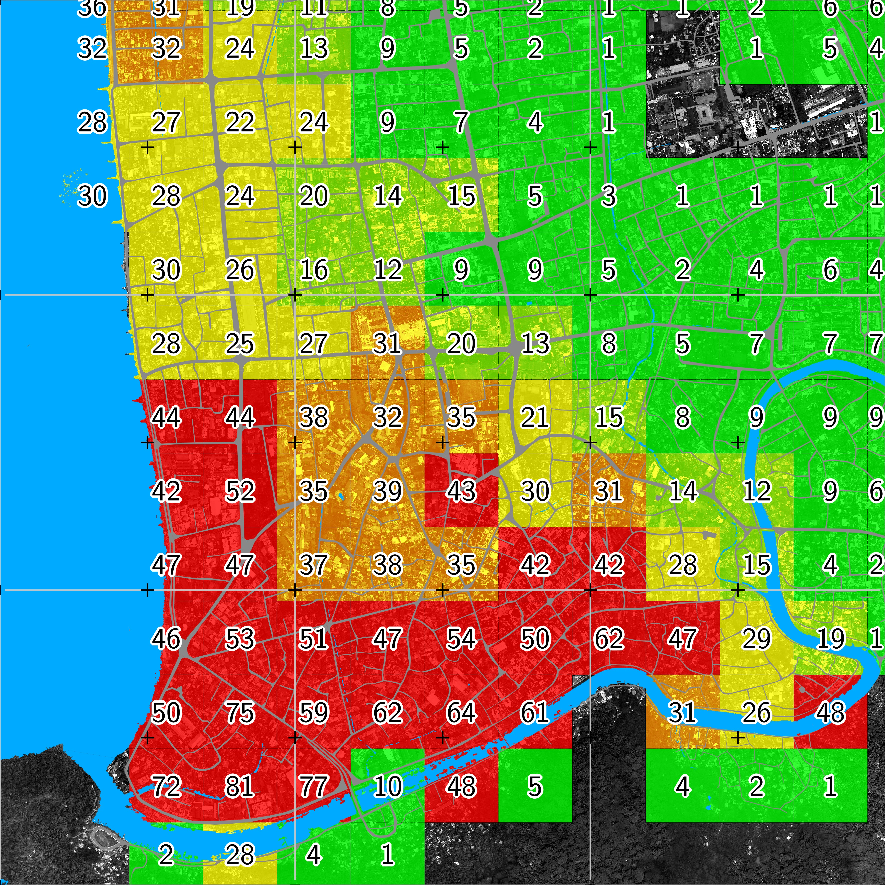
\includegraphics[width=.6\linewidth]{using/figures/dwntwnpdg}
%\caption{Evacuation time analysis for downtown Padang. Numbers showing average evacuation time in mintues, which are also indicated by the colors green, yellow, red.}\label{chap:using:padang}
%\end{figure}
\createfigure%
{Evacuation time analysis for downtown Padang. Numbers showing average evacuation time in mintues, which are also indicated by the colors green, yellow, red.}%
{Evacuation time analysis for downtown Padang. Numbers showing average evacuation time in mintues, which are also indicated by the colors green, yellow, red.}%
{\label{chap:using:padang}}%
{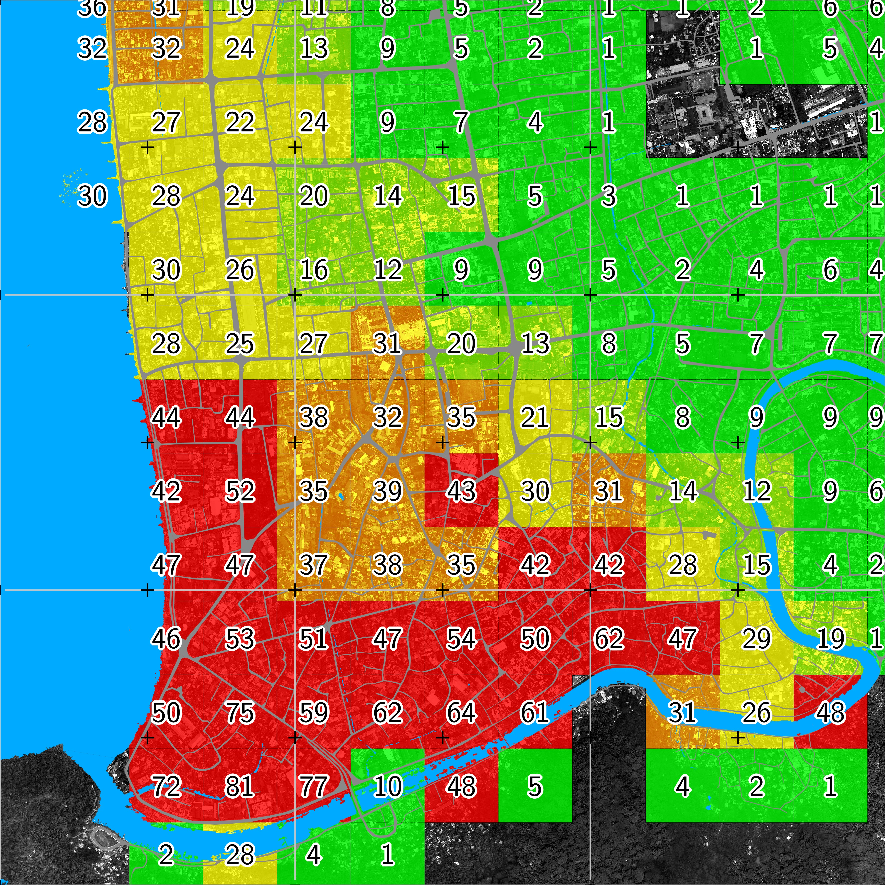
\includegraphics[width=0.6\textwidth, angle=0]{using/figures/dwntwnpdg}}%
{}

Key facts about the Padang scenario:
\begin{itemize}
\item The network consist of about 6,000 nodes and 17,000 links.
\item Synthetic populations for morning, afternoon, and night time have been create comprising up to 330,000 agents.
\item The flooding is modeled by a set of 109 network change events (one per minute) effecting 7609 links.
\item A set of 42 shelter buildings, which can be used for vertical evacuation are also part of the scenario.
\end{itemize}
Based on the Padang scenario various evacuation strategies have been investigated:
\begin{itemize}
\item An obvious evacuation strategy is the shortest path solution, where everyone is on the shortest path. This solution, however, ignores possible congestion and lead to unfeasible results;
\item  An improvement is the so-called Nash equilibrium approach, where everyone tries to find an optimal evacuation route by iterative learning~\citep{LaemmelKluepfelNagel2009EvacPadangAtBookTimmermanns};
\item While the Nash equilibrium reduces the individual evacuation time, the total evacuation might not be minimal. The marginal social cost based simulation approach tries to minimize the total evacuation time~\citep{LaemmelFloetteroed_MertschingEtAl_2009,DresslerFloetteroedLaemmelNagelSkutella2010OptimalEvacuationLargeScaleScenarios};
\item This three basic evacuation approaches are investigated in combination with flooding~\citep{LaemmelEtAl_TransResC_2010};
\item On top of this an evacuation strategy that reduces the risk of exposure is developed by~\citep{LaemmelKluepfelNagel2010PEDRiskPrinted};
\item And finally, \citet{FloetteroedLaemmel2010ICECShelterEvac} propose a method for integrating shelter buildings, which constiitute sinks with limited capacity, into the simulation.  
\end{itemize}
 \cleardoublepage

% ==================================================================================================================
% ##################################################################################################################
\subsection{Patna}
\label{ch:scenarios:patna}
\hfill \textbf{Author:} Amit Agarwal

% ################################################################################################################## \cleardoublepage

% ==================================================================================================================
% ##################################################################################################################
\section{The Philippines: Agent-Based Transport Simulation Model for Disaster Response Vehicles}
\label{sec:philippines}
\hfill \textbf{Author:} Elvira B. Yaneza

% ##################################################################################################################
The primary purpose of this study is to adopt an agent-based traffic simulation model to assist planning agencies in determining road traffic routes for exclusive use of \gls{drv} in the event of disaster. After the initial period of disaster, road network management is crucial to cope with the increase of travel demand for disaster response operations. Depending on the level of road damages, possible road closures may occur in the road network. The degraded road traffic routes of \gls{drv} will result in increase of travel time period from its source to destination.

The model is developed using agent-based simulation modeling paradigm implemented through the use of \gls{matsim}. Road traffic routes are generated using Dijkstra’s shortest path algorithm. \gls{matsim} output files store the routes by each agent. These routes represent the traffic routes for \gls{drv}, in which the travel time calculated in each route is equivalent to the running time of each agent in actual motion while traversing the shortest paths from source to destination. 

% ##################################################################################################################
\section{Literature Review}
Studies involving road traffic routing has generally use different modeling approaches and shortest path algorithms. Among studies using modeling approach, \citet[][]{LefebvreBalmer_TechRep_IVT_2007} used \gls{matsim} for \gls{largescale} agent-based transport simulation and investigated the variations of Dijkstra’s algorithm and A*-algorithm as well. Sumalee and Kurauchi [2] used Monte-Carlo simulation approach to approximate the capacity reliability of the network. The study was then used to evaluate the performances of traffic regulation policies with road network of Kobe city in Japan. Teknomo [3] multi-agent simulation modeling approach considered route probability as direct output of the simulation rather than an input to the network. Sanders and Schultes [4] outlined algorithms for route planning in transportation networks that run faster than Dijkstra’s algorithm. Their study focused on successful speedup techniques in static road network with fixed edge cost. Elalouf [5] model incorporated joint analysis of expected route time and its variance and used dynamic-programming shortest path algorithm as basis for a fully polynomial time approximation scheme. 

% ##################################################################################################################
\section{Design Details And Specifications}
% ..........................................
\paragraph{Element 1: Study Area}
During the occurrence of Tropical Storm Washi (Sendong), the most affected areas were those near the strip of Cagayan de Oro river [6]. Landslides near the river banks, flash floods, overflowing rivers and tributaries, caused some barangays having swept away during the occurrence of Tropical Depression Shanshan (Crising) [7]. The five major bridges mostly affected lie along Cagayan de Oro River connecting its two main lands, District 1 to the west and District 2 to the east, located in the province of Misamis Oriental, Philippines (see Figure~\ref{fig:philippines_fig1}). The designated road network coverage has a total area of approximately 73.2\.square kilometers which includes the riverside (see Figure~\ref{fig:philippines_fig3}). 

% ..........................................
\paragraph{Element 2: Road Network and Facilities}
The model involves three main entities: road network, facilities and population. Road network is described by two variables: nodes and links. It is represented using graphical representation and has 3\,847\,nodes and 9\,630\,directed links (see Figure~\ref{fig:philippines_fig2}). A stretch of a particular street may consist of nodes and links representing intersections and street sections, respectively. \gls{matsim} handles only one-way links. In this model, one-way attribute has a default value of 1 and modes attribute assigned only as car. Facilities are represented by its geographical coordinate locations in the network. It involves twenty one entities from the following agencies: 10\,hospitals with ambulance services, 3\,fire stations, 8\,police stations and 2\,evacuation centers. Facilities are mapped on its nearest links located in the road network.

% ..........................................
\paragraph{Element 3: Population and Demand Generation}
The population is composed of different types of \gls{drv} representing the major agents in the traffic simulation model. These are ambulances, fire trucks and police cars.  The hospitals, fire stations and police stations are assigned as origins of agents, where vehicles start and end their activities, whereas evacuation centers are assigned as destinations of agents. Population is characterized by four variables: person, plan, act and leg. The leg variable is characterized by mode that defines the type of vehicle, assigned as car. The model advances by performing traffic routing activities. Each traffic routing activity, seven events are processed in the following sequence: end activity event, agent departure event, wait to link event, enter link event, leave link event, agent arrival event and start activity event. The end activity event initiates the agent to depart from the facility of origin and back again in the same flow of events. 

% ##################################################################################################################
\section{Model Scenarios} \ah{do we need to use a different term than scenario here? However, these are \emph{actually} scenarios.}
The simulation model was applied to the network of Cagayan de Oro City in Philippines. Two scenarios were assumed.

% ..........................................
\paragraph{Scenario 1: No Bridge Closures}
The scenario was based on disaster response operations right after the occurrence of disaster. The operations took place in Cagayan de Oro City. The scenario has two evacuation centers identified, (1) Balulang Elementary School Evacuation Area located at the west side of Cagayan de Oro and (2) Burgos Barangay Hall Area located at the east side of the city. The road network has 21\,facilities as origins of agents having 3 to 4\,\gls{drv} in each, traversing the network into 2\,different evacuation centers. A total of 67\,\gls{drv} joined the operations over the time and 50\,additional vehicles coming from private institutions traveling on their own rescue operations with different origins and destinations. No road obstructions were considered so traffic movements can access all five bridges defined in the network (see Figure~\ref{fig:philippines_fig4}). During the simulation run, \gls{drv} were expected to pass the nearest bridge on its trip to the destinations or evacuation areas. Thus, passing only the routes that gave shortest time traveled.

% ..........................................
\paragraph{Scenario 2: With Bridge Closures}
In this scenario, road obstructions were represented as bridge closures in the network. The link ids of the identified bridges for closure were required as the data needed to run the java class for road closure generation. In the experiment performed, the link ids of the following three bridges were entered; Carmen Bridge, Rotunda Bridge and Marcos Bridge. The same two evacuation areas and fifty additional vehicles were considered in the experiment. This time considering road obstructions of three bridges only. The \gls{drv} and other vehicles were expected to pass only to the two remaining bridges not included in the road closure generation; Taguanao Bridge and Kauswagan-Puntod Bridge. The expectation of vehicle movements was met as seen during the visualization of the output (see Figure~\ref{fig:philippines_fig5}). 

% ##################################################################################################################
\section{Validation} 
% ..........................................
\paragraph{Face Validation from Field Experts}
The goal was to verify and validate if the simulation model had a reasonable representation of the real-world system and its conformance in the design and operational behavior specifications. Four domain experts were invited from the field of traffic engineering, computing, planning and management for the face validation. Two evaluators were invited from the academe, one was a Transportation Engineering and Built Environment Specialist and the other was a Computing Scientist. The other two evaluators were from the local government units, one was handling management and administration as Technical Supervisor from Road and Traffic Administration Office and the second was involved in planning as Coordinator of Cagayan de Oro City Planning Office. Either accepting or rejecting, the field experts evaluated the simulation model in terms of reasonableness based on their field of expertise. Generally, the four evaluators verified and accepted the design specifications of the simulation model as well as validated and accepted the operational behavior of the simulation model.

% ..........................................
\paragraph{Travel Time Validation Using Test Car Technique and Simulation Model Results}
Looking at the plans file, from both scenarios, it was found out that the calculated travel time resulted from the simulation was actually equal to the amount of running time that the vehicle was in actual motion. The running time was computed as equal to the difference between the travel time and stopped time delay. Actual measurement of travel time and delay using test car technique [8] and travel time using the simulation model were compared. Delay time was the time lost by traffic due to traffic friction, traffic control devices and geometric designs. The actual running time computed was only 36\,\% from the actual total travel time measured due to the amount of travel time delay. The difference between the actual running time computed and running time resulted from the simulation model was mainly caused by the vehicle speed ranges. 

% ##################################################################################################################
\section{Achieved Results}
% ..........................................
\paragraph{Scenario 1: No Bridge Closures}
Based on the generated events file, there were 667\,directed links used by agents representing the \gls{drv}. It was about 6.9\,\% of the total 9\,630\,directed links in the network. The events file stored all activities of 117\,agents, 67\,agents represented the \gls{drv} and 50\,agents represented the additional other vehicles. Finally, when no bridge obstruction occurred, the \gls{drv} coming from 86\,\% of the entities passed by the Carmen Bridge. For faster road traffic access, it was suggested that Carmen Bridge shall be declared exclusive for \gls{drv} during disaster response together with the 667\,directed links.

% ..........................................
\paragraph{Scenario 2: With Bridge Closures}
Results showed that there were 841\,directed links used by agents representing the \gls{drv}, about 8.7\,\% of the total 9\,630\,directed links in the network. Note that three bridges (i.e.,\,Marcos Bridge, Carmen Bridge and Rotunda Bridge) were considered for road closures. \gls{drv} originated from 90\,\% of the entities passed by Kauswagan-Puntod Bridge. Therefore, it was suggested that this bridge and the 841\,directed links were potential candidates in declaring routes for exclusive use of \gls{drv}.

% ################################################################################################################## 
\section{Conclusions}
This study shows that the simulation model has a reasonable representation of the real-world system as verified and validated by the four field domain experts. The results of the study prove the exclusive traffic routing system through the shortest path routes generated by Dijkstra’s algorithm. The results can then be utilized by traffic management decision-makers in determining traffic routes for exclusive use of disaster response vehicles in disaster events.

% ##################################################################################################################
\paragraph{Acknowledgements}
The author wishes to acknowledge the guidance and information received from the developers of \gls{matsim}, Prof. Dr. Nagel Kai of Transport Systems Planning and Transport Telematics at the Institute for Land and Sea Transport Systems, in Berlin, Germany and Dr. Marcel Rieser of Senozon AG in Switzerland. The author would also like to thank Engr. Gerardo S. Doroja for several discussions we had in the implementation of this model.

% ##################################################################################################################
\createfigure%
{Cagayan de Oro City, Philippines urban road network}%
{Cagayan de Oro City, Philippines urban road network}%
{\label{fig:philippines_fig1}}%
{\includegraphics[width=0.85\textwidth, angle=0]{./using/figures/philippines_fig1.png}}%
{GIS City Planning Office, 2012}

\createfigure%
{Spatial coverage of the road network and locations of facilities in the network}%
{Spatial coverage of the road network and locations of facilities in the network: It has 73.2\,square kilometers which includes the land and surrounding river and coastal areas. The facilities are mapped based on its actual geographical x and y coordinates in the road network. There are 23\,facilities located in its nearest link in the network. These are 10\,hospitals, 3\,fire stations, 8\,police stations and 2\,evacuation centers.}%
{\label{fig:philippines_fig3}}%
{\includegraphics[width=0.85\textwidth, angle=0]{./using/figures/philippines_fig3.png}}%
{}

\createfigure%
{Nodes and links representation}%
{Nodes and links representation: Road Network has 3\,837\,nodes representing road intersections and 9\,630\,links representing the streets. It includes five major bridges along Cagayan River: A. Kauswagan-Puntod Bridge, B. Maharlika Bridge (formerly known as Marcos Bridge), C. Gov. Ysalina Bridge (formerly known as Carmen Bridge), D. Kagay-an Bridge (Rotunda Bridge) and E. Emmanuel Pelaez Bridge.}%
{\label{fig:philippines_fig2}}%
{\includegraphics[width=0.85\textwidth, angle=0]{./using/figures/philippines_fig2.png}}%
{}

\createfigure%
{Screenshot of SCENARIO~1}%
{Screenshot of SCENARIO~1 (without bridge closures) using agent~ID\#4. \protect\gls{drv} trip starting from the Sabal Hospital (Origin) passing Carmen Bridge (Gov. Ysalina Bridge) going to Balulang Evacuation Center dropping point (destination) then back to its origin.}%
{\label{fig:philippines_fig4}}%
{\includegraphics[width=0.85\textwidth, angle=0]{./using/figures/philippines_fig4.png}}%
{}

\createfigure%
{Screenshot of SCENARIO~2}%
{Screenshot of SCENARIO~2 (with bridge closures) using Agent~ID\#48. \protect\gls{drv} trip starting from the Sabal Hospital (Origin) passing Kauswagan-Puntod Bridge going to Balulang Evacuation Center dropping point (destination) then back to its origin.}%
{\label{fig:philippines_fig5}}%
{\includegraphics[width=0.85\textwidth, angle=0]{./using/figures/philippines_fig5.png}}%
{}

% ##################################################################################################################






 
 \cleardoublepage

% ==================================================================================================================
% ##################################################################################################################
\section{Poznan}
\label{sec:poznan}
\hfill \textbf{Author:} Michal Maciejewski

% ################################################################################################################## \cleardoublepage

% ==================================================================================================================
% ##################################################################################################################
\section{Quito Metropolitan District}
\label{sec:quito}
\hfill \textbf{Authors:} Rolando Armas, Hernán Aguirre

% ##################################################################################################################
\gls{dmq}, Ecuador, has grown rapidly the last years increasing traffic congestion, gas emissions, pollution, and use of energy. Our research integrates evolutionary computation, traffic simulation, emission models, and data mining tools to gain a better understanding on \gls{dmq}’s complex mobility and transportation system and propose solutions to it from a sustainability standpoint.

As a first case study \citep[][]{ArmasEtAl_SEAL_2014}, we have implemented a mobility scenario to optimize traffic lights under congested conditions. We have focused on the
\gls{dmq}’s business district, which geographical area covers 7x3\,square kilometers as shown in Figure~\ref{fig:quito_fig1}. The area considers only the primary and secondary pathways, which free speeds are in the range from 30 to 80\,kilometers per hour. The network has 1\,000\,links approximately and comes from Geofabrik and \gls{osm}. The number of simulated agents is 20\,000. The mobility plan for each agent consists of three main trips: (1) home to work, (2) work to leisure, and (3) leisure to home (see Figure~\ref{fig:quito_fig2}). The plans are designed so that all agents move first from south to north, completely crossing the geographical area of study. In their second trip, the agents move from north to the central zone of the area under study and in their last trip from the central zone to the south. Eleven signal lights are located in a main two-way street with flows in south-north and north-south directions (see Figure~\ref{fig:quito_fig1}).

The evolutionary algorithm finds optimal signal settings of the \gls{dmq} scenario minimizing average travel time. First, we run \gls{matsim} for 500\,iterations, making sure it reaches a user equilibrium state without setting any traffic signal. After that, the evolutionary algorithm evolves a population of candidate solutions for a number of generations. Each solution represents a configuration of signals (signal control) for the transportation system. At each generation, the evolutionary algorithm calls \gls{matsim} for each candidate solution in order to evaluate it. \gls{matsim} starts from the equilibrium state setting its signals controls with the tentative solution provided by the optimizer and runs one additional iteration. The output collected from that iteration of the simulator is used to calculate travel time, which is passed as fitness of the solution to the optimizer. Figure~\ref{fig:quito_fig2} illustrates the interaction of \gls{matsim} and the evolutionary algorithm. The first case study \citep[][]{ArmasEtAl_SEAL_2014} provides valuable insights to understand better the optimal setting of traffic lights in the business district of \gls{dmq} under congested conditions, allows us to validate the problem representation used in the evolutionary algorithm and the effectiveness of the mutation and recombination operators implemented to search solutions.

Currently, we are scaling up the number of traffic signals to be optimized and testing under other mobility scenarios within the same area of study. Our next step is to incorporate a emissions model and use multi- and many-objective evolutionary algorithms \citep[][]{AguireEtAl_EMO_2013} to evolve optimal designs of the transportation and mobility system of the \gls{dmq} satisfying multiple criteria for sustainability. These criteria include desired transportation and mobility policies, accessibility, reduction of emissions, reduction of energy use, and societal and economic benefit.

\createfigure%
{Study area}%
{Study area}%
{\label{fig:quito_fig1}}%
{\includegraphics[width=0.7\textwidth, angle=0]{./using/figures/qfig1.png}}%
{}

\createfigure%
{Optimization system}%
{Optimization system}%
{\label{fig:quito_fig2}}%
{\includegraphics[width=0.7\textwidth, angle=0]{./using/figures/qfig2.png}}%
{}

% ##################################################################################################################


 \cleardoublepage

% ==================================================================================================================
% ==================================================================================================================
\section{Rotterdam: Revenue Management in Public Transportation with Smart-Card Data Enabled Agent-Based Simulations \textsuperscript{\footnotesize{\footnote{This research was conducted at Rotterdam School of Management and
supported by Netherlands Organisation for Scientific Research (NWO)
Complexity Grant No. 645.000.001 awarded to Dr. Ting Li and Prof.mr.dr. Peter Vervest from
Rotterdam School of Management. It was presented at \protect\gls{matsim} User Meetings in 2011 and 2012,
INFORMS International 2012 Beijing, the 7th Workshop on Agents in Traffic and Transportation at
AAMAS 2012 Valencia, Erasmus University Rotterdam, Berlin Institute of Technology, Tsinghua
University and Beijing Jiaotong University.}}}}
\label{sec:rotterdam}
\hfill \textbf{Authors:} Paul Bouman, Milan Lovric

% ==================================================================================================================
In \citet[][]{LovricEtAl_DSS_2013} and \citet[][]{BoumanEtAl_AAMAS_2012}, we proposed two scenarios for studying revenue management in public transportation via time-based pricing strategies, such as peak markups and off-peak discounts, nowadays being used by various transit agencies. To evaluate this approach, we developed agent-based simulations using \gls{matsim} and a transportation demand generated from smart-card data collected in a Dutch urban area. In the first scenario, we simulated only a metro network, while in the second scenario we considered a \gls{multimodal} network consisting of metro, tram and bus.

In \citet[][]{LovricEtAl_DSS_2013}, we designed and implemented a decision support system for sustainable revenue management that can evaluate the impact of various revenue management strategies on economic, social, and environmental performance. Figure~\ref{fig:rotterdam} shows the structure of the decision support system built on top of the \gls{matsim} framework. Smart card transactions (individual check-in and check-out transactions made at stations' entrance and exit gates) were used to reconstruct daily tours of individual passengers. These were inputted into \gls{matsim} as the initial demand. Furthermore, information about the transit network and vehicle schedule was extracted from the \gls{osm} data and the public transit operator's web site, respectively. Revenue management experiments were then conducted by applying various time-based pricing strategies defined as percentage-wise discounts or markups (applied on top of the nominal price) during specific periods of the day. 

\gls{matsim}'s loop (Section~\ref{sec:inbrief}) was adapted for studying time-based pricing. Firstly, an event handler was created to calculate travel fare of the whole daily tour for each individual (this was implemented according to the real-life pricing scheme: a fixed fee applied at check-in plus a variable distance-based fee applied at check-out). Secondly, we adapted the original Charypar-Nagel scoring function \citep[][]{CharyparNagel2005ga4acts} by adding the disutility of the travel fare. The existing \gls{matsim}'s time mutator was used as a replanning strategy to allow passengers to discover more affordable travel times when pricing strategies were enforced (however, a trade-off was introduced by applying a penalty for arriving outside of the expected arrival window that was based on the check-out times observed in the smart card data).

To capture the impact of revenue management on the three sustainability dimensions, we added event handlers to produce a number of relevant \glspl{kpi}. The economic performance was measured by the revenue of the \gls{pto}, passenger kilometers, and vehicle load factors. The social performance was measured by the availability of seating places (as a proxy for passenger comfort) calculated from vehicles loadings after the mobility simulation. We also looked at the average tour price as the measure of public transportation affordability. The impact of a pricing policy on the environment was expressed as the change in carbon footprint stemming from a possible shift of demand between public transportation and private cars (calculated from the change in average tour price and the elasticity of demand). 

Our results show that, by using a smart-card enabled decision support system and by taking a customer-centric view, \glspl{pto} can better explore the space of feasible solutions in a broader policy-making context that includes all three dimensions of people-profit-planet sustainability. We validated our approach by comparing the simulation-generated travel fares in the nominal scenario with actual fares recorded in the smart card transactional database \citep[see][]{LovricEtAl_DSS_2013}.

To further study the opportunities of smart card data for demand generation, in paper by \citet[][]{BoumanEtAl_AAMAS_2012} we introduced a pattern-based demand generation method using smart card transactions of three different modalities (metro, tram and bus) in an urban area of The Netherlands as an input. In addition to the use of observations for a single day to generate activity-based demand, daily commuting patterns detected from longitudinal observations for a single smart card were generated. In the specific study, the generated demands were utilized to analyze time-shifting behavior under two different revenue management policies: a plain tariff (with a fixed price per journey and a price per unit of traveled distance) and an off-peak discount. The experiment was repeated for different amounts of pattern-based demand, where the varied parameter was the number of observed samples required for a smart card to be included. 

In the generated demand, the agents which were not generated using pattern-based demand had to replicate their observed tour or trip within 15\,minute windows of the observed arrival and departure times. The pattern-based agents had time windows dependent on the observed standard deviations in passengers' actual commuting travel patterns, which were used as a proxy for their time flexibility. This aspect of the demand modeling was more detailed than in study of \citet[][]{LovricEtAl_DSS_2013}, in which agents were assumed homogeneous with respect to their time flexibility. This flexibility was exploited by the time shift mutator which was made available in \gls{matsim} as one of the \gls{replanning} strategies. In future work, improvements in the scoring function and the use of more sophisticated pattern-based demand generation approach need to be considered in order to create more realistic scenarios for a study of time-shifting behavior under revenue management policies.

\createfigure%
{Rotterdam scenario: Decision support system for sustainable revenue management in public transportation}%
{Rotterdam scenario: Decision support system for sustainable revenue management in public transportation}%
{\label{fig:rotterdam}}%
{\includegraphics[width=0.85\textwidth, angle=0]{./using/figures/rotterdam}}%
{}

% ==================================================================================================================

 \cleardoublepage

% ==================================================================================================================
% ##################################################################################################################
\section{San Francisco Bay Area}
\label{sec:sf}
\hfill \textbf{Author:} Alexey Pozdnukhov

% ################################################################################################################## ok \cleardoublepage

% ==================================================================================================================
% ##################################################################################################################
\section{Seattle Region}
\label{sec:seattle}
\hfill \textbf{Author:} Kai Nagel

% ##################################################################################################################
A \gls{matsim} model of the Seattle region---more precisely of the \gls{psrc} area---was developed during a sabbatical stay of K.\ Nagel with the \gls{urbansim} team in Seattle in 2008. The model resulted from a prototypical integration of the \gls{urbansim} software \citep[e.g.,][]{WaddellEtc2003UrbanSim} with \gls{matsim}. 

The base was an existing \gls{psrc} \gls{urbansim} model, which used an existing \gls{emme2} model 
%\kai{citation!} \ah{Etwa so? \citep[][]{RolleEtAl_ITE_2007, EMME_Webpage_2008}} \kai{Ja danke.  ausser dass ich das Rolle paper nicht kenne; hoffe, es geht über emme :-)} 
as a travel model. It was investigated how difficult it would be to replace the \gls{emme2} model by \gls{matsim}. 

The network was taken by conversion from the existing \gls{emme} network, resulting in 15\,478\,links and 5\,025\,nodes with attributes length, free speed, and capacity.

The demand was generated as output from \gls{urbansim}. Evidently, the \gls{urbansim} simulation already contained a full synthetic population of the area. The \gls{urbansim} model was also set up with workplace choice, so that each synthetic person with status "working" had a workplace assigned. Since that version of \gls{urbansim} worked on the parcel level, this meant that home-to-work trips could be extracted directly, with coordinates, from the model. As so often for initial \gls{matsim}  studies, this home-to-work demand was completed into home-work-home plans.

The configuration used the standard \gls{matsim} scoring parameters, a workplace opening time of 7\,am, and a latest work start time of 9\,am. The iterations were run with re-routing and time mutation enabled until convergence. Since this was an exercise in rapid prototyping, only a 1\,\% sample of the full synthetic population was used; the flow and storage capacities of the road network were scaled down accordingly. Figure~\ref{fig:seattle-snapshot.left} shows a result. Figure~\ref{fig:seattle-snapshot.right} shows households most affected by a hypothetical closure of the Alaskan Way viaduct, which bypasses the Seattle downtown area on the waterfront side to the west.
%
\createfigure%
{Seattle region scenario}%
{Seattle region scenario}%
{\label{fig:seattle-snapshot}}%
{%
  \createsubfigure%
  {Simulated congestion patterns in Seattle at 7:30\,am}%
  {\includegraphics[width=0.49\textwidth,angle=0]{using/figures/seattle-snapshot-7h30.pdf}}%
  {\label{fig:seattle-snapshot.left}}%
  {}%
  \createsubfigure%
  {10\,\% households most affected by closure of the so-called Alaskan Way Viaduct (in red)}%
	{\includegraphics[width=0.49\textwidth,angle=0]{using/figures/seattle-top-10pct-0it.pdf}}%
  {\label{fig:seattle-snapshot.right}}%
  {}%
}%
{}

% ##################################################################################################################


% Local Variables:
% mode: latex
% mode: reftex
% mode: visual-line
% TeX-master: "../../main"
% comment-padding: 1
% fill-column: 9999
% End: 
 \cleardoublepage

% ==================================================================================================================
% ##################################################################################################################
\subsection{Seoul}
\label{ch:scenarios:seoul}
\hfill \textbf{Author:} Seungjae Lee

<sjlee@uos.ac.kr> zugesagt

% ################################################################################################################## \cleardoublepage

% ==================================================================================================================
% ##################################################################################################################
\subsection{Shanghai}
\label{ch:scenarios:shanghai}
\hfill \textbf{Author:} Lun angeschrieben

\citep[][]{WangtEtAl_TRB_2013}

% --------
\paragraph{Associated projects:}

% --------
\paragraph{Study area:}

% --------
\paragraph{Population and demand generation:}

% --------
\paragraph{Activity Locations:}

% --------
\paragraph{Network:}

% --------
\paragraph{Modes:}

% --------
\paragraph{Calibration and validation:}

\ah{Simulation quality, achieved results}

% ################################################################################################################## \cleardoublepage

% ==================================================================================================================
% ##################################################################################################################
\section{Sochi}
\label{ch:scenarios:sochi}
\hfill \textbf{Author:} Marcel Rieser




% ################################################################################################################## \cleardoublepage

% ==================================================================================================================
% ##################################################################################################################
\chapter{Stockholm}
\label{ch:stockholm}
\hfill \textbf{Author:} Joschka Bischoff

\editdone{This text has undergone the professional edit. Please no grammatical changes anymore! They are most-probably wrong.}

% ##################################################################################################################
The Stockholm scenario was created as a student project at TU Berlin in summer, 2014. 
Because several groups worked on the project, the common base was a census data synthetic population, an \gls{osm}-based network and counts data.

The network was taken from \gls{osm} 2013~data. 
Within the city, all roads were used; in outlying regions, only mayor roads were included in the network. 
Demand consisted of home-work-home-plans only. 
The population sample size was---depending on the student group---between 1 and 5\,\%. Agents used car and (pseudo) public transit.

Count data for the morning peak along a mayor road, the E4, was used to calibrate the scenario. 
This calibration was handled differently by the groups; some just added traffic, others tried to imitate the Stockholm toll. 
Further scenario documentation is available in German. 

% ##################################################################################################################
 \cleardoublepage

% ==================================================================================================================
% ##################################################################################################################
\section{Tampa}
\label{ch:scenarios:tampa}
\hfill \textbf{Author:} Sashikanth Gurram


% ################################################################################################################## \cleardoublepage

% ==================================================================================================================
% ##################################################################################################################
\section{Tel Aviv}
\label{ch:scenarios:telaviv}
\hfill \textbf{Author:} Christoph Dobler

\citep[][]{BekhorEtAl_TRB_2011}

% ################################################################################################################## \cleardoublepage

% ==================================================================================================================
% ##################################################################################################################
\section{Toronto}
\label{sec:toronto}
\hfill \textbf{Author:} Adam Weiss, Peter Kucireck, Khandker Nurul Habib

% ##################################################################################################################
\subsection{Study Area:}
The Greater Toronto and Hamilton Area (GTHA) is situated to the north west of Lake Ontario in the province of Ontario, forming Canada’s largest urban region. The GTHA’s current population is over 6.5\,million, with projected growth to approximately 8.6\,million by 2031. 

% =============================================================================================
\subsection{Population, Demand Generation and Activity locations}
The Transportation Tomorrow Survey (TTS) forms the basis of the travel demand to be used for the multimodal assignment simulation. The TTS is a retrospective telephone survey conducted in the GTHA every 5\,years. The TTS samples just over 5\,\% of the GTHA households. The survey collects household socioeconomic and geographical characteristics, characteristics of each household member, and a full 24\,hours travel diary for each household member. The current MATSIM models use the TTS travel diary records to generate the plans file. There has also been some investigation into the integration of the Travel Activity Scheduler for Household Agents (TASHA) activity based model, which has been developed for the GTHA. Irrespective of the source of the demand data, both sources provide the traffic zone location of all activities. The Toronto implementation will then randomly distribute the activities around the traffic zone, resulting in unique x-y coordinates for each activity. Within the current implementation of MATSIM within Toronto, no development of MATSIM facilities has been attempted.

% =============================================================================================
\subsection{Network Development and Simulated Modes}  
The GTHA MATSIM implementation uses a preexisting planning level network for static user equilibrium assignment using the EMME traffic assignment software. This network is converted to a MATSIM network using a conversion tool, which can be found in the MATSIM Toronto playground. More recently, this network was merged with GTFS data for 5 of the 8\,major regional transit agencies to allow for multimodal demand assignment.  

% =============================================================================================
\subsection{Calibration, Validation, Results}
The Toronto MATSIM implementation has been compared to the more conventional large-scale assignment models with varying degrees of success. While the work of \citet[][]{GaoWEtAl_TRR_2010}, found that travel time, travel distance, link flows and speeds were all reasonably comparable and in fact more plausible than those achieved through the EMME assignment. Conversely, work on transit assignment done first by \citet[][]{Kucirek_MastersThesis_2012} and then by \citet[][]{WeissEtAl_CJCE_2012} found that there were limitations associated with predicting line boardings based on different transit technologies and agencies, which utilized different fare structure, suggesting that further work to calibrate the multimodal assignment model is required. These issues are exasperated by the current implementations inability to distinguish between in vehicle dwell times and out of vehicle wait times, which ideally should be weighted differently, particularly given the climate and prominence of outdoor bus stops within the region. 

% =============================================================================================

% ################################################################################################################## \cleardoublepage

% ==================================================================================================================
% ##################################################################################################################
\section{Trondheim}
\label{ch:scenarios:trondheim}
\hfill \textbf{Authors:} Stefan Fl�gel, Julia Kern 


% ################################################################################################################## \cleardoublepage

% ==================================================================================================================
\section{Yarrawonga and Mulwala: Demand-responsive transportation in regional Victoria, Australia}
\label{sec:yarrawonga}
\hfill \textbf{Author:} Nicole Ronald
% ==================================================================================================================

In November 2013, Public Transport Victoria (PTV) implemented a service called
Flexiride in twin towns in regional Victoria, consisting of an on-demand public
transport service using taxis. This service replaced an existing fixed-route bus
service, which had a low patronage.

The aim of this scenario was to investigate the change in operational
performance between two different DRT schemes: the Flexiride scheme and a
completely ad-hoc scheme. More details can be found in
\citep[][]{RonThoWin2015}. This work is a first step towards developing a
decision-support tool to evaluate different DRT schemes, in particular
integrated with other modes of transport. 


% --------
%Associated projects: 
The scenario was built as part of a larger project exploring the viability of
mobility-on-demand, focusing on ridesharing and demand-responsive transportation
(DRT) services \citep[][]{Ronald_iMoD_2014}.

% --------
%Study area: 
The scenario covers twin towns on the border of Victoria and New South Wales,
Australia, separated by the Murray River. Yarrawonga (Victoria) has a population
of 7,057 and an area of 95.0km$^2$, while Mulwala (New South Wales) has a
population of 1,904 and an area of 18.6km$^2$. 

The Flexiride scheme delivers six services on weekdays and three services on
Saturday, leaving the centre of Yarrawonga (Orr St) at fixed times.  The local
taxi operator is paid a holding fee by PTV to ensure that a taxi is available at
Orr St at the nominated time. The taxi returns to normal service if there are no
bookings and no passengers waiting.

Passengers can ride either by booking over the phone at least 10 minutes before
the service is scheduled to depart from Orr St, or by arriving at Orr St in
person to begin their trip. Existing bus stops were used as pickup and dropoff
points.

Figure \ref{fig:yarrawonga} shows the stops in both towns; the main stop
in Yarrawonga, Orr St, is denoted by a star.

\createfigure%
{Location of bus stops in Yarrawonga/Mulwala}%
{Location of bus stops in Yarrawonga/Mulwala, including origin/destination zones}%
{\label{fig:yarrawonga}}%
{\includegraphics[width=0.85\textwidth, angle=0]{./using/figures/yarrawonga_high.png}}%
{}


% --------
%Population and demand generation:

Flexiride drivers record the location of pickups and drop-offs for each service,
as well as fare revenue collected. Using this data, probabilities of trips
occurring between two zones were developed following the process in
\citep[][]{Deflorio_ITSIET_2011}. A continuous distribution of departure times was
derived from evenly spreading the demand for particular services to either side
of that service. 

% --------
%Activity Locations: not used

% --------
%Network:
The network was extracted from OpenStreetMap. Some bus stops were removed if
they were assigned to the same link in MATSim, e.g., stops on the same road
between intersections.

% --------
%Modes:
Only passengers for the demand-responsive service are included. However, the use
of MATSim for this initial model means that we can add in other modes for later
versions.

% --------
%Calibration and validation: exploratory

% --------
%Simulation quality and achieved results:
This was an exploratory simulation, intended to demonstrate how DRT can be
modeled for exploring viability and how different schemes can be compared.

Using MATSim, experimentation with varying demands, two different scheduling
algorithms, and an altered Flexiride service with more services was able to be
carried out. Outcomes such as drive time, vehicle-kilometres traveled, and
passenger wait time could be measured.

Results showed that the two schemes performed differently for operators and
passengers. Optimization schemes had little effect with low demands, while
seating requirements showed more variability in the ad-hoc scheme as demand
increased. Future work involves estimating costs of the two schemes for further
comparison.


% --------
%Miscellaneous, important to mention:

% --------
%Specialties:

%-------
% Acknowledgements:

This work has been supported by a grant from the Australian Research Council
(LP120200130). We are also grateful to Michal Maciejewski for his assistance
with the dvrp module. Michael Rigby prepared the map of Yarrawonga and Mulwala.
% ================================================================================================================== \cleardoublepage

% ==================================================================================================================
%Further models are available or currently being developed \citep[][]{Axhausen_unpub_Hong_Kong_2013, MATSIM-T-Scenarios_Webpage_2014}: 
% Izmir, 'yalcin.alver@ege.edu.tr'; 'mmetinm@gmail.com' 
% Aliaga, 'pelin.onelcin@ege.edu.tr'
% Caracas, 'hector.navarro@ciens.ucv.ve'
% Boading (China), Chengxiang Zhuge, Chunfu Shao, Jian Gao, Meng Meng and Weiyang Xu: 'gaojian615@126.com'; 'zgcx615@126.com'; 'xutryever@126.com'; 'cfshao@bjtu.edu.cn'; 'weiyangxu23@126.com'
% Ivory Coast (Zilske), 
% LA (Balmer, unfinished), 
% Kyoto (who?)
% Santiago (who?)
% all contacted, where possible.

% ##################################################################################################################
%\section{Discussion and TODOs}
%Will be commented, when chapter is finished. Make final results traceable.

%\ah{
%- region description (characteristics, stats, ...)
%- population (popgen, Balmi plug together)
%- facilities
%- network
%- utility function (estimated, how derived)
%- pt (simulated, pseudo pt)
%- modes
%- freight (siehe keynotes Kai)
%- border crossers/boundary effects
%
%data sources
%methods applied
%
%- special problems faced \& solutions found
%
%- simulation quality
%- calibration \& validation (+available data)
%
%- purpose and sponsor/client
%- associated projects -> see Section \ref{sec:projects}
%
%- specialties: parataxis in Gauteng, connections to other sims (Toronto, Tel-Aviv)
%}

% ##################################################################################################################
